% The preamble has been dumped out as out/presentationpreamble.fmt file. You can recreate that file by
% xelatex -ini -jobname="presentationpreamble" -output-directory=out "&xelatex presentationpreamble.tex\dump"
\documentclass[10pt, compress]{beamer}
\usetheme[usetitleprogressbar]{m}
 
 \usepackage{booktabs} % for better tables
 \usepackage{natbib}  % for better citations
 \usepackage{media9} % for includemedia i.e. videos
 \usepackage{xcolor} % for more colors
 
\usepackage{tikz}
\usetikzlibrary{shadows,trees}
\usetikzlibrary{shapes,calc,backgrounds}
\usetikzlibrary{fadings}
\usepackage{tikz3d}
\usepgfplotslibrary{dateplot}
\usepackage{graphicx}

% New math commands/abreviations

\newcommand{\bA}{\mathbf{A}}
\newcommand{\bB}{\mathbf{B}}
\newcommand{\bC}{\mathbf{C}}
\newcommand{\bD}{\mathbf{D}}
\newcommand{\bE}{\mathbf{E}}
\newcommand{\bF}{\mathbf{F}}
\newcommand{\bG}{\mathbf{G}}
\newcommand{\bH}{\mathbf{H}}
\newcommand{\bI}{\mathbf{I}}
\newcommand{\bJ}{\mathbf{J}}
\newcommand{\bK}{\mathbf{K}}
\newcommand{\bL}{\mathbf{L}}
\newcommand{\bM}{\mathbf{M}}
\newcommand{\bN}{\mathbf{N}}
\newcommand{\bO}{\mathbf{O}}
\newcommand{\bP}{\mathbf{P}}
\newcommand{\bQ}{\mathbf{Q}}
\newcommand{\bR}{\mathbf{R}}
\newcommand{\bS}{\mathbf{S}}
\newcommand{\bT}{\mathbf{T}}
\newcommand{\bU}{\mathbf{U}}
\newcommand{\bV}{\mathbf{V}}
\newcommand{\bW}{\mathbf{W}}
\newcommand{\bX}{\mathbf{X}}
\newcommand{\bY}{\mathbf{Y}}
\newcommand{\bZ}{\mathbf{Z}}

\newcommand{\ba}{\mathbf{a}}
%\newcommand{\bb}{\mathbf{b}}
\newcommand{\bc}{\mathbf{c}}
\newcommand{\bd}{\mathbf{d}}
\newcommand{\be}{\mathbf{e}}
%\newcommand{\bf}{\mathbf{f}}
\newcommand{\bg}{\mathbf{g}}
\newcommand{\bh}{\mathbf{h}}
\newcommand{\bi}{\mathbf{i}}
\newcommand{\bj}{\mathbf{j}}
\newcommand{\bk}{\mathbf{k}}
\newcommand{\bl}{\mathbf{l}}
%\newcommand{\bm}{\mathbf{m}}
\newcommand{\bn}{\mathbf{n}}
%\newcommand{\bo}{\mathbf{o}}
\newcommand{\bp}{\mathbf{p}}
\newcommand{\bq}{\mathbf{q}}
\newcommand{\br}{\mathbf{r}}
\newcommand{\bs}{\mathbf{s}}
\newcommand{\bt}{\mathbf{t}}
\newcommand{\bu}{\mathbf{u}}
\newcommand{\bv}{\mathbf{v}}
\newcommand{\bw}{\mathbf{w}}
\newcommand{\bx}{\mathbf{x}}
\newcommand{\by}{\mathbf{y}}
\newcommand{\bz}{\mathbf{z}}

\newcommand{\bff}{\mathbf{f}}

\newcommand{\bo}{\mathbf{0}}
\newcommand{\tx}{\tilde{\mathbf{x}}}


\newcommand{\hbn}{{\widehat{\mathbf{n}}}}
\newcommand{\hbs}{{\widehat{\mathbf{s}}}}
\newcommand{\hbh}{{\widehat{\mathbf{h}}}}
\newcommand{\hbv}{{\widehat{\mathbf{v}}}}
\newcommand{\hbw}{{\widehat{\mathbf{w}}}}
\newcommand{\hbc}{{\widehat{\mathbf{c}}}}

\newcommand{\hh}{{\widehat{h}}}
\newcommand{\hn}{{\widehat{n}}}
\newcommand{\hx}{{\widehat{x}}}
\newcommand{\hy}{{\widehat{y}}}
\newcommand{\hz}{{\widehat{z}}}


% Mathcal definitions
\newcommand{\cS}{\mathcal{S}}
\newcommand{\cD}{\mathcal{D}}
\newcommand{\cP}{{\mathcal{P}}}
\newcommand{\cU}{{\mathcal{U}}}
\newcommand{\cV}{{\mathcal{V}}}
\newcommand{\cE}{{\mathcal{E}}}
\newcommand{\cQ}{{\mathcal{Q}}}
\newcommand{\cG}{{\mathcal{G}}}
\newcommand{\cB}{{\mathcal{B}}}
\newcommand{\cI}{\mathcal{I}}
\newcommand{\cL}{\mathcal{L}}
\newcommand{\cR}{{\mathcal{R}}}
\newcommand{\cC}{{\mathcal{C}}}
\newcommand{\cO}{{\mathcal{O}}}
\newcommand{\cX}{{\mathcal{X}}}



% Mathbb definitions
\newcommand{\bbp}{\mathbb{P}}
\newcommand{\bbP}{\mathbb{P}}
\newcommand{\bbQ}{\mathbb{Q}}
\newcommand{\bbr}{\mathbb{R}}
\newcommand{\bbR}{\mathbb{R}}
\newcommand{\bbS}{\mathbb{S}}
\newcommand{\bbN}{\mathbb{N}}



% Mathbm definitions
\newcommand{\balpha}{{\bm{\alpha}}}
\newcommand{\bbeta}{{\bm{\beta}}}
\newcommand{\bgamma}{{\bm{\gamma}}}
\newcommand{\bmu}{{\bm{\mu}}}
\newcommand{\bpi}{\bm{\pi}}
\newcommand{\brho}{\bm{\rho}}
\newcommand{\bomega}{\bm{\omega}}
\newcommand{\bOmega}{\bm{\Omega}}
\newcommand{\bSigma}{\bm{\Sigma}}
\newcommand{\bGamma}{\bm{\Gamma}}



\newcommand{\id}{\mathbf{I}}
\newcommand{\tid}{\tilde{\id}}
\newcommand{\st}{{\textrm{subject to }}}


\newcommand{\bpm}{{\widehat{\bP}}}
\newcommand{\bxm}{{\widehat{\mathbf{X}}}}
\newcommand{\winf}{{{\bm{\Omega}}_\infty}}
%\newcommand{\bw}{{{\bm{\omega}}^*}}
\newcommand{\bwi}{{{\bm{\omega}}_i^*}}
\newcommand{\bwone}{{{\bm{\omega}}_1^*}}
\newcommand{\diac}{{{\bm{\omega}}^*}}
\newcommand{\iac}{{{\bm{\omega}}}}
\newcommand{\ac}{{{\bm{\Omega}}_\infty}}
\newcommand{\diaci}{{{\bm{\omega}}_i^*}}
\newcommand{\diacone}{{{\bm{\omega}}_1^*}}
\newcommand{\w}{{{\bm{\omega}}^*}}
\newcommand{\daq}{{\mathbf{Q}}_\infty^*}
\newcommand{\adq}{{\mathbf{Q}}_\infty^*}
\newcommand{\pinf}{{\bm{\pi}}_\infty}
\newcommand{\hinf}{{{\bH}_\infty}}
\newcommand{\hinft}{{{\bH}^\top_\infty}}
\newcommand{\hinfi}{{{\bH}^i_\infty}}
\newcommand{\hinfit}{{{\bH}^{i\top}_\infty}}
\newcommand{\hinfj}{{{\bH}^j_\infty}}
\newcommand{\hinfjt}{{{\bH}^{j\top}_\infty}}
\newcommand{\intval}[2]{[\, #1, #2 \, ]}
\newcommand{\camo}{\left[ \: \id \: \vert \: \bo \: \right]}
\newcommand{\cama}{\left[ \: \bA \: \vert \: \ba \: \right]}
\newcommand{\camr}{\left[ \: \bR \: \vert \: \bt \: \right]}
\newcommand{\camai}{\left[ \: \bA_i \: \vert \: \ba_i \: \right]}
\newcommand{\camri}{\left[ \: \bR_i \: \vert \: \bt_i \: \right]}

%\newcommand{\algorithmiccomment}[1]{//#1}
\newcommand{\lb}{\operatorname{\bf{Bound}}}
\newcommand{\branch}{\operatorname{\bf{Branch}}}
\newcommand{\feasible}{\operatorname{\bf{Feasible}}}
\newcommand{\trace}{\operatorname{Tr}}
\newcommand{\convenv}{\operatorname{\bf{convenv}}}
\newcommand{\rectangle}{Q}

\newcommand{\epi}{\operatorname{\bf{epi}}}
\newcommand{\dom}{\operatorname{\bf{dom}}}

\newcommand{\ophi}{f}
\newcommand{\phimin}{\ophi_{\text{min}}}
\newcommand{\philb}{\ophi_{\text{lb}}}
\newcommand{\phiub}{\ophi_{\text{ub}}}

\newcommand{\cvx}{{\mathrm{convex\_env}}}
\newcommand{\ccv}{{\mathrm{concave\_env}}}

\newcommand{\conc}[1]{\operatorname{conc}{#1}}
\newcommand{\conv}[1]{\operatorname{conv}{#1}}

%\newcommand{\deg}[1]{\operatorname{deg}{#1}}

\newcommand{\lmi}[1]{\operatorname{LMI}{#1}}

\newcommand{\fa}{\alpha}
\newcommand{\fb}{\beta}
\newcommand{\fc}{\gamma}


%\newcommand{\tr}{^\top}

\newcommand{\xlt}{x_l^{1/3}}
\newcommand{\xut}{x_u^{1/3}}
\newcommand{\tlt}{t_l^{1/3}}
\newcommand{\tut}{t_u^{1/3}}
\newcommand{\xl}{x_l}
\newcommand{\xu}{x_u}
\newcommand{\yl}{y_l}
\newcommand{\yu}{y_u}
\newcommand{\tl}{t_l}
\newcommand{\tu}{t_u}
\newcommand{\yp}{y_p}
\newcommand{\ypd}{y'_p}
\newcommand{\tp}{t_p}
\newcommand{\fl}{\frac{x - \xl}{\xu - \xl}}
\newcommand{\fu}{\frac{\xu - x}{\xu - \xl}}


% Bilinear definitions
\newcommand{\cl}{{\psi}^l}
\newcommand{\cu}{{\psi}^u}
\newcommand{\rect}{Q}
\newcommand{\cond}[1]{\operatorname{{\mathcal{C}}}{#1}}
\newcommand{\vol}[1]{\operatorname{vol}{#1}}

%\newcommand{\phimin}[1]{\operatorname{\Phi_{\textrm{min}}}{#1}}
%\newcommand{\philb}[1]{\operatorname{\Phi_{\textrm{lb}}}{#1}}
%\newcommand{\phiub}[1]{\operatorname{\Phi_{\textrm{ub}}}{#1}}


%\newcommand{\rank}{{\mathbf{rank}}}
%\newcommand{\diag}{{\mathrm{diag}}}

\newcommand{\rank}[1]{\operatorname{rank}{#1}}

%\newcommand{\bx}{x} %general unknown x
%\newcommand{\bX}{X} %scene point

\newcommand{\ix}{\bx} %image point
\newcommand{\ixa}{u} %1st coordinate of image point
\newcommand{\ixb}{v} %2nd coordinate of image point
\newcommand{\bXa}{U} %1st coordinate of scene point
\newcommand{\bXb}{V} %2nd coordinate of scene point
\newcommand{\bXc}{W} %3rd coordinate of scene point

\newcommand{\tr}{^\top}

\newcommand{\Linf}{L_{\infty}}
\newcommand{\Ltwo}{L_{2}}
\newcommand{\Lone}{L_{1}}
\newcommand{\Lp}{L_{p}}
\newcommand{\Lq}{L_{q}}

\def\smallmat#1{\left[\begin{smallmatrix}#1\end{smallmatrix}\right]}



\newcommand{\brs}{\bR_0}
\newcommand{\bts}{\bt_0}
\newcommand{\bzero}{\mathbf{0}}
\newcommand{\bdx}{\mathbf{dx}}

\newcommand{\p}{\partial}


\newcommand{\del}[1]{\nabla_{#1}}
\newcommand{\I}{\mathbf{I}}
\newcommand{\II}{\mathbf{II}}
\newcommand{\skewsymm}[1]{[{#1}]_\times}





% 3D pose of the cars and ego motion
\newcommand{\pos}[2]{\mathbf{p}^{#1}({#2})}
\newcommand{\ori}[2]{\mathbf{\omega}^{#1}(#2)}
\newcommand{\state}[2]{\mathbf{s}^{#1}(#2)}

% ego pose
\newcommand{\egop}[1][t]{\pos{c}{#1}}
\newcommand{\egoo}[1][t]{\ori{c}{#1}}
\newcommand{\egos}[1][t]{\state{c}{#1}}

% relative pose between camera and car $i$
\newcommand{\relp}[2]{\Omega^{(#1)}(#2)}
\newcommand{\relpz}[2]{\Omega_z^{(#1)}(#2)}

% 3D tracks on car $i$ in its own coordinate frame
\newcommand{\tracklets}{\mathbf{X}^{(i)}_o}
\newcommand{\tracklet}[1]{\mathbf{x}^{(i)}_{#1}}
% track projections on camera
\newcommand{\trackpit}[2]{\mathbf{u}^{(#1)}(#2)}
\newcommand{\trackp}[1]{\mathbf{u}^{(j)}(#1)}
\newcommand{\trackpj}[1]{\mathbf{u}_j(#1)}
% Unclassified track point projected on camera
\newcommand{\ucTrackp}{\mathbf{u}(t)}


% dimensions of car $i$
\newcommand{\dimsn}[1]{\mathbf{B}^{(#1)}}
\newcommand{\expDimsn}{\hat{\mathbf{B}}}

% projection function
\newcommand{\projectionOf}[1]{\pi_{\relp{i}{t}}\left(#1\right)}
\newcommand{\projectionOft}[1]{\pi_{\relp{i}{t+1}}\left(#1\right)}
\newcommand{\centerProj}{\bar{\pi}_{\relp{i}{t}}(\dimsn{i})}
\newcommand{\cornerProj}[1]{\pi^{#1}_{\relp{i}{t}}(\dimsn{i})}
\newcommand{\triangleProj}[1]{\triangle^{#1}_{\relp{i}{t}}(\dimsn{i})}

% bounding box corners on image
\newcommand{\bbt}[2]{\mathbf{d}^{(#1)}({#2})}
\newcommand{\bb}[1]{\mathbf{d}^{(#1)}(t)}


\newcommand{\Energy}[1]{\mathcal{E}^{it}_{\text{#1}}}
\newcommand{\pEnergy}[1]{\mathcal{E}^{ijt}_{\text{#1}}}
% Weighted energy
\newcommand{\WEnergy}[1]{\lambda_{\text{#1}}\Energy{#1}}
\newcommand{\WpEnergy}[1]{\lambda_{\text{#1}}\pEnergy{#1}}
\newcommand{\EnergyCol}{\mathcal{E}^{ijt}_{\text{col}}}
\newcommand{\WEnergyCol}{\lambda_{\text{col}}\EnergyCol}

\newcommand{\EnergyBBoxNoOcc}{\pEnergy{bboxNoOcc}}
\newcommand{\EnergyBBox}{\pEnergy{bbox}}
\newcommand{\EnergyTrack}{ \pEnergy{track}}
\newcommand{\EnergyTrackNoOcc}{\pEnergy{trackNoOcc}}
\newcommand{\EnergyLane}{\Energy{lane}}
\newcommand{\EnergySize}{\Energy{size}}
\newcommand{\EnergyDyn}{\Energy{dyn}}
\newcommand{\EnergyDynHol}{\Energy{dyn-hol}}
\newcommand{\EnergyDynOri}{\Energy{dyn-ori}}
\newcommand{\EnergyDynVel}{\Energy{dyn-vel}}

\newcommand{\occFreeProj}[1]{\Pi_{\relp{i}{t}}(#1)}
\newcommand{\minx}{x_{\text{min}}}
\newcommand{\miny}{y_{\text{min}}}
\newcommand{\maxx}{x_{\text{max}}}
\newcommand{\maxy}{y_{\text{max}}}
\newcommand{\frontface}{F^i_\text{FF}(t)}

\newcommand{\occ}[1]{o({#1})}
\newcommand{\face}{F^i_k(t)}

\newcommand{\invProjectionOf}[1]{\pi^{-1}_{\relp{i}{t}}\left(#1\right)}
\newcommand{\invProjectionOftm}[1]{\pi^{-1}_{\relp{i}{t-1}}\left(#1\right)}
\newcommand{\occf}{f^i_{occ}(\mathbf{x}_j)}
\newcommand{\occftot}{f_{occ}(\mathbf{x}_j)}
\newcommand{\occft}[1]{f_{occ}(#1)}

\newcommand{\ray}{\hat{\mathbf{r}}_j}
\newcommand{\occfray}{f_{occ}(\lambda\ray)}
\newcommand{\lambdadist}{f_{\lambda}(\trackpj{t-1}, \lambda)}

\newcommand{\occfxi}{L(\mathbf{x}; \pos{i}{t-1}, \Sigma_i)}
\newcommand{\occfi}{L(\lambda \ray; \pos{i}{t-1}, \Sigma_i)}
\newcommand{\assocP}{a^{(ij)}(\lambda)}
\newcommand{\assocPk}{a^{(ij)}(\lambda_k)}

\newcommand{\Ereproj}{E^{(ij)}_{\text{reproj}}}
\newcommand{\Ptransarg}[1]{P^{(j)}_{\text{transmission}}(#1)}
\newcommand{\Ptrans}{\Ptransarg{\lambda}}
\newcommand{\Ptransmud}{P^{(j)}_{\text{transmission}}(\mu^{(i)}_d)}
\newcommand{\Prefl}{P^{(ij)}_{\text{reflection}}(\lambda)}
\newcommand{\dishort}{d_i(\mathbf{x})}

\newcommand{\Lu}{L_u(\mathbf{u}, \mu^i_u,\Sigma^i_u)}
\newcommand{\Llambda}{L_{\lambda}(\mathbf{u}, \lambda; \mu^i_d)}

\newcommand{\Gauss}{\mathcal{N}}
\newcommand{\PropDist}{\mathcal{W}_j}

\newcommand{\muijl}{\mu^{(ij)}_{\lambda}}
\newcommand{\sigmaijl}{\sigma^{ij}_{\lambda}}

\newcommand{\Sigmait}{\Sigma^{(i)^{-1}}_t}

\newcommand{\muit}{\mu^{(i)}_t}
\newcommand{\Sigmaic}{\Sigma'^{(i)^{-1}}_c}

\newcommand{\muic}{{\mu^{(i)}_c}}
\newcommand{\Sigmaicf}{\Sigma^{(i)^{-1}}_c}

\newcommand{\muiu}{\mu^{(i)}_t}
\newcommand{\Sigmaiu}{\Sigma^{(i)^{-1}}_u}

\newcommand{\uv}[1]{\hat{\mathbf{#1}}}
\newcommand{\Tr}[3]{{}^{#1}{#2}_{#3}}
\newcommand{\xymin}[1]{#1_{\text{min}}}
\newcommand{\xymax}[1]{#1_{\text{max}}}
\newcommand{\vect}[1]{\mathbf{#1}}
\newcommand{\map}{\vect{x}}

\newcommand{\xt}{\mathbf{x}_t}
\newcommand{\xc}{\mathbf{x}_c}

\newcommand{\Rctot}{R}
\newcommand{\tctot}{t}

\newcommand{\tcmut}{t'}


\newcommand{\Beizer}{B\'eizer }

\newcommand{\LaneUncertainty}[1]{\Sigma_{L_m}(#1)}
\newcommand{\projOnLane}[1]{\pi_{L_m(k)}(#1)}


%\DeclareMathSymbol{\Tangent}
\DeclareMathOperator{\diag}{diag}
\DeclareMathOperator{\sech}{sech}
\DeclareMathOperator{\poly}{poly}
%\DeclareMathOperator*{\argmin}{\arg\min}




\providecommand{\dscale}{0.5}
% Image frame
\newcommand{\drawframe}{
  %\path[use as bounding box,draw] (0.5,-2) rectangle (10,2);

\coordinate (A\x) at (\x*1.2,0);
\coordinate (a\x) at (\x*1.2+0.3,0+0.5);

\draw [thick,black] (A\x) -- +(0,1) -- +(1,1.5) -- +(1,.5) -- cycle;


\draw [very thick,blue!40,fill=blue!20] (a\x) -- +($\dscale*(0,1)$) node (b\x) {} -- +($\dscale*(1,1.5)$) node (c\x) {} -- +($\dscale*(1,.5)$) node (d\x) {} -- cycle;

}

\newcommand{\road}{
    % Road width
    \newcommand{\rw}{0.15};
    % Road slant
    \newcommand{\rslant}{0.15};
    % Upper coordinate of the road
    \pgfmathsetmacro{\rup}{\rw+\rslant};
    % Where does the road start on the left
    \newcommand{\rxmin}{6};
    % length of the  road
    \newcommand{\rxlen}{5};
    % right end of the road
    \pgfmathsetmacro{\rxmax}{\rxmin+\rxlen};

    % Draw the road
    \filldraw[fill=black!20, draw=black!40] 
    (3d cs:\rxmin, 0,  0) -- (3d cs:\rxmax, 0, \rslant)
    -- (3d cs:\rxmax, 0,  \rup) -- (3d cs:\rxmin, 0, \rw) -- cycle;
    % Middle of the road coordinates
    \pgfmathsetmacro{\rmid}{\rw/2};
    \pgfmathsetmacro{\rmidr}{\rslant + (\rw)/2};
    % Dashed line in the middle of the road
    \draw[white,very thick,dashed] (3d cs:\rxmin, 0, \rmid ) -- (3d cs:\rxmax, 0, \rmidr);
}

\newcommand{\acuboid}{
  \providecommand{\acxmin}{-2}
  \providecommand{\acxlen}{1}
  \providecommand{\acymin}{-2}
  \providecommand{\acylen}{1}
  \providecommand{\aczmin}{-2}
  \providecommand{\aczlen}{1}
  \pgfmathsetmacro{\acymax}{\acymin+\acylen}
  \pgfmathsetmacro{\acxmax}{\acxmin+\acxlen}
  \pgfmathsetmacro{\aczmax}{\aczmin+\aczlen}
  \coordinate (a) at (3d cs:\acxmax,\acymax,\aczmin);
  \coordinate (b) at (3d cs:\acxmax,\acymax,\aczmax);
  \coordinate (c) at (3d cs:\acxmax,\acymin,\aczmax);
  \coordinate (d) at (3d cs:\acxmax,\acymin,\aczmin);
  \coordinate (h) at (3d cs:\acxmin,\acymin,\aczmin);
  \coordinate (e) at (3d cs:\acxmin,\acymax,\aczmin);
  \coordinate (f) at (3d cs:\acxmin,\acymax,\aczmax);

  \draw [facestyle] (a) -- (b) -- (c) -- (d) -- cycle;
  \draw [facestyle] (a) -- (b) -- (f) -- (e) -- cycle;
  \draw [facestyle] (a) -- (d) -- (h) -- (e) -- cycle;
  % For debugging turn this on to see corners labeled
  %\path (a) node {a} (b) node {b} (c) node {c} (d) node {d}  (h) node {h} (e) node {e} (f) node {f};
}

\newcommand{\car}{
\providecommand{\cxmin}{0}
\providecommand{\cxmax}{1}
\providecommand{\czmin}{0}
\providecommand{\czmax}{1}
\providecommand{\cyzmin}{0}
\providecommand{\cyzmax}{0}
\providecommand{\cylen}{1}
    \path (3d cs:\cxmin, 0, \czmin) coordinate (a)
    (3d cs:\cxmax, 0, \czmax) coordinate (b)
    (3d cs:\cxmax, \cylen, \czmax) coordinate (c)
    (3d cs:\cxmin, \cylen, \czmin) coordinate (d)
    (3d cs:\cxmax, \cylen, \cyzmax) coordinate (e)
    (3d cs:\cxmin, \cylen, \cyzmin) coordinate (f)
    (3d cs:\cxmin, 0, \cyzmin) coordinate (g)
    ;

  % front face
  \filldraw[facestyle] (a) -- (b) -- (c) --  (d) -- cycle;
  % upper face
  \filldraw[facestyle] (c) -- (e) -- (f) --  (d) -- cycle;
  % left (wrt viewer) face
  \filldraw[facestyle] (a) -- (d) -- (f) --  (g) -- cycle;
  \node (lB) at ($(e) + (0,.2)$) {$\dimsn{i}$};
}

\newcommand{\caronroad}{
  % Draw the road and the car
  \begin{scope}[3d/perspective eye={0,5,-1},facestyle/.style={fill=blue!20, draw=blue!40}]    
    %\path[use as bounding box,clip] (5.5,-1) rectangle (8,3);
    \road{}

    % Displacement of car w.r.t road
    \newcommand{\cxdisp}{1};
    % left most coordinate of the car
    \pgfmathsetmacro{\cxmin}{\cxdisp+\rxmin};
    % length of car
    \newcommand{\cxlen}{1.5};
    % height of car
    \newcommand{\cylen}{.8};
    % width of car
    \newcommand{\czlen}{.4*\rw};
    % right most x-coordinate of car
    \pgfmathsetmacro{\cxmax}{\cxmin+\cxlen};
    % z-min coordinate of car
    \pgfmathsetmacro{\czmin}{\rslant/\rxlen*\cxdisp+0.02};
    % z-max
    \pgfmathsetmacro{\czmax}{\rslant/\rxlen*(\cxmax-\rxmin)+0.02};
    % z-max on the farther side
    \pgfmathsetmacro{\cyzmax}{\czmax+\czlen};
    % z-min on the farther side
    \pgfmathsetmacro{\cyzmin}{\czmin+\czlen};

    \car{}
  \end{scope}
}

% Camera
\newcommand{\camera}{
\path (5,1) coordinate (c0) 
 +(0.25,0.15) coordinate (c2);
  \draw (c0) rectangle (c2);
  \draw (c2) -- ++(0.075, 0.075) -- ++(0, -0.3) -- ++(-0.075,0.075) ;
}


\def\interminputs#1#2#3#4#5{
  ($(o) + (hgap)$) node[data] (det) {Detections #1}
  +(vgap) node[data] (pt) {Point Tracks #2}
  +($2*(vgap)$) node[data] (gp) {Ground plane #3}
  +($3*(vgap)$) node[data] (ego) {Egomotion #4}
  +($4*(vgap)$) node[data] (lane) {Lanes #5}
}

\newlength{\units}
\setlength{\units}{0.8cm}
\def\beginproblemflowchartsetup{
  \begin{tikzpicture}[
      every edge/.style = {very thick,>=stealth,draw,red,->},
      data/.style = {rectangle,rounded corners,fill=blue!20,draw,
      minimum width=3\units},
    algo/.style = {rectangle,fill=red!20,draw}]
    \coordinate (hgap) at (3.5, 0);
    \coordinate (vgap) at (0, -1);
    \coordinate (o) at (0,0);
   %\path[draw,use as bounding box] ($5*(vgap)-0.5*(hgap)$) rectangle ($-0.5*(vgap)+3*(hgap)$);
  }
\def\endproblemflowchartsetup{ \end{tikzpicture} }
\def\systemandout#1{
    \path 
    ($(o)+2*(vgap)+2*(hgap)$) node [algo] (os) {Our system}
    +($0.8*(hgap)$) node [data,align=left] (out) {3D localization\\ and dimensions #1};
}
\def\rawtointerm{
    \path (mv) edge (det);
    \path (mv) edge (pt);
    \path (mv) edge (gp);
    \path (mv) edge (ego);
    \path (mv) edge (lane);
    \path (gps) edge (lane);
    \path (map) edge (lane);
}
\def\intermtosys{
    \path (det) edge (os);
    \path (pt) edge (os);
    \path (gp) edge (os);
    \path (ego) edge (os);
    \path (lane) edge (os);

    \path (os) edge (out);
}
\newcommand{\problemflowchart}[5]{
  \beginproblemflowchartsetup
    \path 
    ($(o)+2*(vgap)$) node[data] (mv) {Mono-Video}
    ++($1.5*(vgap)$) node[data] (gps) {GPS}
    +($(vgap)$) node[data] (map) {Map};

    \path \interminputs{#1}{#2}{#3}{#4}{#5};

    \begin{pgfonlayer}{background}
      % Left-top corner of the background rectangle
      \path (det.east |- det.north)+(0.25,0.25) node (a) {};
      % Right-bottom corner of the background rectanle
      \path (mv.west |- map.south)+(-0.25,-0.25) node (c) {};
      % Draw the background
      \path[fill=green!20,rounded corners, draw=green,thick]
      (a) rectangle (c);
      \node at ($(det) - (hgap)$) {Inputs};
    \end{pgfonlayer}


    %\path[use as bounding box,draw] (map.south west) rectangle ($(out.east |- det.north)+(0.25,0.25)$);
    \systemandout{}


    \rawtointerm
    \intermtosys
  \endproblemflowchartsetup
}
\newcommand{\problemflowchartnoraw}[7]{
  \beginproblemflowchartsetup

    \path \interminputs{#1}{#2}{#3}{#4}{#5};

    \node (inp) at ($(det) - 0.8*(vgap)$) {Inputs #7};
    \begin{pgfonlayer}{background}
      % Left-top corner of the background rectangle
      \path (gp.east |- inp.north)+(0.25,0.25) node (a) {};
      % Right-bottom corner of the background rectanle
      \path (gp.west |- lane.south)+(-0.25,-0.25) node (c) {};
      % Draw the background
      \path[fill=green!20,rounded corners, draw=green,thick]
      (a) rectangle (c);
    \end{pgfonlayer}

    \systemandout{#6}

    \intermtosys

    \node [anchor=north west,align=left] (oseq) at ($(os)+2*(vgap)$) {\normalsize{$ \{\state{i}{t}\}^* = \arg \max_{\{\state{i}{t}\}} P(\{\state{i}{t}\} | \mathbb{E})\enspace. $}};
    \draw [->,very thick,green!50!black] (os) -- (oseq);
  \endproblemflowchartsetup
}

\newcommand{\colcol}{\color{blue}}
\newcommand{\colbbox}{\color{green!50!black}}
\newcommand{\coltrack}{\color{red}}
\newcommand{\collane}{\color{cyan}}
\newcommand{\colsize}{\color{magenta}}
\newcommand{\coldyn}{\color{orange}}
\let\oldWEnergyCol\WEnergyCol
\renewcommand{\WEnergyCol}{{\colcol\oldWEnergyCol}}
\newcommand{\WEnergyBBox}{{\colbbox\WpEnergy{bbox}}}
\newcommand{\WEnergyTrack}{{\coltrack\WpEnergy{track}}}
\newcommand{\WEnergyTrackNoOcc}{{\coltrack\WpEnergy{trackNoOcc}}}
\newcommand{\WEnergyLane}{{\collane\WEnergy{lane}}}
\newcommand{\WEnergySize}{{\colsize\WEnergy{size}}}
\newcommand{\WEnergyDyn}{{\coldyn\WEnergy{dyn}}}

\let\oldEnergyCol\EnergyCol
\renewcommand{\EnergyCol}{\colcol\oldEnergyCol}

\providecommand{\EnergyBBoxNoOcc}{{\colbbox\pEnergy{bboxNoOcc}}}
\providecommand{\EnergyBBox}{{\colbbox\pEnergy{bbox}}}
\providecommand{\EnergyTrack}{{\coltrack \pEnergy{track}}}
\providecommand{\EnergyTrackNoOcc}{{\coltrack\pEnergy{trackNoOcc}}}
\providecommand{\EnergyLane}{{\collane\Energy{lane}}}
\providecommand{\EnergySize}{{\colsize\Energy{size}}}
\providecommand{\EnergyDyn}{{\coldyn\Energy{dyn}}}
\providecommand{\EnergyDynHol}{{\coldyn\Energy{dyn-hol}}}
\providecommand{\EnergyDynOri}{{\coldyn\Energy{dyn-ori}}}
\providecommand{\EnergyDynVel}{{\coldyn\Energy{dyn-vel}}}
\renewcommand{\EnergyBBoxNoOcc}{{\colbbox\pEnergy{bboxNoOcc}}}
\renewcommand{\EnergyBBox}{{\colbbox\pEnergy{bbox}}}
\renewcommand{\EnergyTrack}{{\coltrack \pEnergy{track}}}
\renewcommand{\EnergyTrackNoOcc}{{\coltrack\pEnergy{trackNoOcc}}}
\renewcommand{\EnergyLane}{{\collane\Energy{lane}}}
\renewcommand{\EnergySize}{{\colsize\Energy{size}}}
\renewcommand{\EnergyDyn}{{\coldyn\Energy{dyn}}}
\renewcommand{\EnergyDynHol}{{\coldyn\Energy{dyn-hol}}}
\renewcommand{\EnergyDynOri}{{\coldyn\Energy{dyn-ori}}}
\renewcommand{\EnergyDynVel}{{\coldyn\Energy{dyn-vel}}}

% 
% To compile you need to load that binary file using -fmt option
% xelatex -fmt out/presentationpreamble.fmt -output-directory=out presentation.tex
%\documentclass[10pt, compress]{beamer}
\usetheme[usetitleprogressbar]{m}
 
 \usepackage{booktabs} % for better tables
 \usepackage{natbib}  % for better citations
 \usepackage{media9} % for includemedia i.e. videos
 \usepackage{xcolor} % for more colors
 
\usepackage{tikz}
\usetikzlibrary{shadows,trees}
\usetikzlibrary{shapes,calc,backgrounds}
\usetikzlibrary{fadings}
\usepackage{tikz3d}
\usepgfplotslibrary{dateplot}
\usepackage{graphicx}

% New math commands/abreviations

\newcommand{\bA}{\mathbf{A}}
\newcommand{\bB}{\mathbf{B}}
\newcommand{\bC}{\mathbf{C}}
\newcommand{\bD}{\mathbf{D}}
\newcommand{\bE}{\mathbf{E}}
\newcommand{\bF}{\mathbf{F}}
\newcommand{\bG}{\mathbf{G}}
\newcommand{\bH}{\mathbf{H}}
\newcommand{\bI}{\mathbf{I}}
\newcommand{\bJ}{\mathbf{J}}
\newcommand{\bK}{\mathbf{K}}
\newcommand{\bL}{\mathbf{L}}
\newcommand{\bM}{\mathbf{M}}
\newcommand{\bN}{\mathbf{N}}
\newcommand{\bO}{\mathbf{O}}
\newcommand{\bP}{\mathbf{P}}
\newcommand{\bQ}{\mathbf{Q}}
\newcommand{\bR}{\mathbf{R}}
\newcommand{\bS}{\mathbf{S}}
\newcommand{\bT}{\mathbf{T}}
\newcommand{\bU}{\mathbf{U}}
\newcommand{\bV}{\mathbf{V}}
\newcommand{\bW}{\mathbf{W}}
\newcommand{\bX}{\mathbf{X}}
\newcommand{\bY}{\mathbf{Y}}
\newcommand{\bZ}{\mathbf{Z}}

\newcommand{\ba}{\mathbf{a}}
%\newcommand{\bb}{\mathbf{b}}
\newcommand{\bc}{\mathbf{c}}
\newcommand{\bd}{\mathbf{d}}
\newcommand{\be}{\mathbf{e}}
%\newcommand{\bf}{\mathbf{f}}
\newcommand{\bg}{\mathbf{g}}
\newcommand{\bh}{\mathbf{h}}
\newcommand{\bi}{\mathbf{i}}
\newcommand{\bj}{\mathbf{j}}
\newcommand{\bk}{\mathbf{k}}
\newcommand{\bl}{\mathbf{l}}
%\newcommand{\bm}{\mathbf{m}}
\newcommand{\bn}{\mathbf{n}}
%\newcommand{\bo}{\mathbf{o}}
\newcommand{\bp}{\mathbf{p}}
\newcommand{\bq}{\mathbf{q}}
\newcommand{\br}{\mathbf{r}}
\newcommand{\bs}{\mathbf{s}}
\newcommand{\bt}{\mathbf{t}}
\newcommand{\bu}{\mathbf{u}}
\newcommand{\bv}{\mathbf{v}}
\newcommand{\bw}{\mathbf{w}}
\newcommand{\bx}{\mathbf{x}}
\newcommand{\by}{\mathbf{y}}
\newcommand{\bz}{\mathbf{z}}

\newcommand{\bff}{\mathbf{f}}

\newcommand{\bo}{\mathbf{0}}
\newcommand{\tx}{\tilde{\mathbf{x}}}


\newcommand{\hbn}{{\widehat{\mathbf{n}}}}
\newcommand{\hbs}{{\widehat{\mathbf{s}}}}
\newcommand{\hbh}{{\widehat{\mathbf{h}}}}
\newcommand{\hbv}{{\widehat{\mathbf{v}}}}
\newcommand{\hbw}{{\widehat{\mathbf{w}}}}
\newcommand{\hbc}{{\widehat{\mathbf{c}}}}

\newcommand{\hh}{{\widehat{h}}}
\newcommand{\hn}{{\widehat{n}}}
\newcommand{\hx}{{\widehat{x}}}
\newcommand{\hy}{{\widehat{y}}}
\newcommand{\hz}{{\widehat{z}}}


% Mathcal definitions
\newcommand{\cS}{\mathcal{S}}
\newcommand{\cD}{\mathcal{D}}
\newcommand{\cP}{{\mathcal{P}}}
\newcommand{\cU}{{\mathcal{U}}}
\newcommand{\cV}{{\mathcal{V}}}
\newcommand{\cE}{{\mathcal{E}}}
\newcommand{\cQ}{{\mathcal{Q}}}
\newcommand{\cG}{{\mathcal{G}}}
\newcommand{\cB}{{\mathcal{B}}}
\newcommand{\cI}{\mathcal{I}}
\newcommand{\cL}{\mathcal{L}}
\newcommand{\cR}{{\mathcal{R}}}
\newcommand{\cC}{{\mathcal{C}}}
\newcommand{\cO}{{\mathcal{O}}}
\newcommand{\cX}{{\mathcal{X}}}



% Mathbb definitions
\newcommand{\bbp}{\mathbb{P}}
\newcommand{\bbP}{\mathbb{P}}
\newcommand{\bbQ}{\mathbb{Q}}
\newcommand{\bbr}{\mathbb{R}}
\newcommand{\bbR}{\mathbb{R}}
\newcommand{\bbS}{\mathbb{S}}
\newcommand{\bbN}{\mathbb{N}}



% Mathbm definitions
\newcommand{\balpha}{{\bm{\alpha}}}
\newcommand{\bbeta}{{\bm{\beta}}}
\newcommand{\bgamma}{{\bm{\gamma}}}
\newcommand{\bmu}{{\bm{\mu}}}
\newcommand{\bpi}{\bm{\pi}}
\newcommand{\brho}{\bm{\rho}}
\newcommand{\bomega}{\bm{\omega}}
\newcommand{\bOmega}{\bm{\Omega}}
\newcommand{\bSigma}{\bm{\Sigma}}
\newcommand{\bGamma}{\bm{\Gamma}}



\newcommand{\id}{\mathbf{I}}
\newcommand{\tid}{\tilde{\id}}
\newcommand{\st}{{\textrm{subject to }}}


\newcommand{\bpm}{{\widehat{\bP}}}
\newcommand{\bxm}{{\widehat{\mathbf{X}}}}
\newcommand{\winf}{{{\bm{\Omega}}_\infty}}
%\newcommand{\bw}{{{\bm{\omega}}^*}}
\newcommand{\bwi}{{{\bm{\omega}}_i^*}}
\newcommand{\bwone}{{{\bm{\omega}}_1^*}}
\newcommand{\diac}{{{\bm{\omega}}^*}}
\newcommand{\iac}{{{\bm{\omega}}}}
\newcommand{\ac}{{{\bm{\Omega}}_\infty}}
\newcommand{\diaci}{{{\bm{\omega}}_i^*}}
\newcommand{\diacone}{{{\bm{\omega}}_1^*}}
\newcommand{\w}{{{\bm{\omega}}^*}}
\newcommand{\daq}{{\mathbf{Q}}_\infty^*}
\newcommand{\adq}{{\mathbf{Q}}_\infty^*}
\newcommand{\pinf}{{\bm{\pi}}_\infty}
\newcommand{\hinf}{{{\bH}_\infty}}
\newcommand{\hinft}{{{\bH}^\top_\infty}}
\newcommand{\hinfi}{{{\bH}^i_\infty}}
\newcommand{\hinfit}{{{\bH}^{i\top}_\infty}}
\newcommand{\hinfj}{{{\bH}^j_\infty}}
\newcommand{\hinfjt}{{{\bH}^{j\top}_\infty}}
\newcommand{\intval}[2]{[\, #1, #2 \, ]}
\newcommand{\camo}{\left[ \: \id \: \vert \: \bo \: \right]}
\newcommand{\cama}{\left[ \: \bA \: \vert \: \ba \: \right]}
\newcommand{\camr}{\left[ \: \bR \: \vert \: \bt \: \right]}
\newcommand{\camai}{\left[ \: \bA_i \: \vert \: \ba_i \: \right]}
\newcommand{\camri}{\left[ \: \bR_i \: \vert \: \bt_i \: \right]}

%\newcommand{\algorithmiccomment}[1]{//#1}
\newcommand{\lb}{\operatorname{\bf{Bound}}}
\newcommand{\branch}{\operatorname{\bf{Branch}}}
\newcommand{\feasible}{\operatorname{\bf{Feasible}}}
\newcommand{\trace}{\operatorname{Tr}}
\newcommand{\convenv}{\operatorname{\bf{convenv}}}
\newcommand{\rectangle}{Q}

\newcommand{\epi}{\operatorname{\bf{epi}}}
\newcommand{\dom}{\operatorname{\bf{dom}}}

\newcommand{\ophi}{f}
\newcommand{\phimin}{\ophi_{\text{min}}}
\newcommand{\philb}{\ophi_{\text{lb}}}
\newcommand{\phiub}{\ophi_{\text{ub}}}

\newcommand{\cvx}{{\mathrm{convex\_env}}}
\newcommand{\ccv}{{\mathrm{concave\_env}}}

\newcommand{\conc}[1]{\operatorname{conc}{#1}}
\newcommand{\conv}[1]{\operatorname{conv}{#1}}

%\newcommand{\deg}[1]{\operatorname{deg}{#1}}

\newcommand{\lmi}[1]{\operatorname{LMI}{#1}}

\newcommand{\fa}{\alpha}
\newcommand{\fb}{\beta}
\newcommand{\fc}{\gamma}


%\newcommand{\tr}{^\top}

\newcommand{\xlt}{x_l^{1/3}}
\newcommand{\xut}{x_u^{1/3}}
\newcommand{\tlt}{t_l^{1/3}}
\newcommand{\tut}{t_u^{1/3}}
\newcommand{\xl}{x_l}
\newcommand{\xu}{x_u}
\newcommand{\yl}{y_l}
\newcommand{\yu}{y_u}
\newcommand{\tl}{t_l}
\newcommand{\tu}{t_u}
\newcommand{\yp}{y_p}
\newcommand{\ypd}{y'_p}
\newcommand{\tp}{t_p}
\newcommand{\fl}{\frac{x - \xl}{\xu - \xl}}
\newcommand{\fu}{\frac{\xu - x}{\xu - \xl}}


% Bilinear definitions
\newcommand{\cl}{{\psi}^l}
\newcommand{\cu}{{\psi}^u}
\newcommand{\rect}{Q}
\newcommand{\cond}[1]{\operatorname{{\mathcal{C}}}{#1}}
\newcommand{\vol}[1]{\operatorname{vol}{#1}}

%\newcommand{\phimin}[1]{\operatorname{\Phi_{\textrm{min}}}{#1}}
%\newcommand{\philb}[1]{\operatorname{\Phi_{\textrm{lb}}}{#1}}
%\newcommand{\phiub}[1]{\operatorname{\Phi_{\textrm{ub}}}{#1}}


%\newcommand{\rank}{{\mathbf{rank}}}
%\newcommand{\diag}{{\mathrm{diag}}}

\newcommand{\rank}[1]{\operatorname{rank}{#1}}

%\newcommand{\bx}{x} %general unknown x
%\newcommand{\bX}{X} %scene point

\newcommand{\ix}{\bx} %image point
\newcommand{\ixa}{u} %1st coordinate of image point
\newcommand{\ixb}{v} %2nd coordinate of image point
\newcommand{\bXa}{U} %1st coordinate of scene point
\newcommand{\bXb}{V} %2nd coordinate of scene point
\newcommand{\bXc}{W} %3rd coordinate of scene point

\newcommand{\tr}{^\top}

\newcommand{\Linf}{L_{\infty}}
\newcommand{\Ltwo}{L_{2}}
\newcommand{\Lone}{L_{1}}
\newcommand{\Lp}{L_{p}}
\newcommand{\Lq}{L_{q}}

\def\smallmat#1{\left[\begin{smallmatrix}#1\end{smallmatrix}\right]}



\newcommand{\brs}{\bR_0}
\newcommand{\bts}{\bt_0}
\newcommand{\bzero}{\mathbf{0}}
\newcommand{\bdx}{\mathbf{dx}}

\newcommand{\p}{\partial}


\newcommand{\del}[1]{\nabla_{#1}}
\newcommand{\I}{\mathbf{I}}
\newcommand{\II}{\mathbf{II}}
\newcommand{\skewsymm}[1]{[{#1}]_\times}





% 3D pose of the cars and ego motion
\newcommand{\pos}[2]{\mathbf{p}^{#1}({#2})}
\newcommand{\ori}[2]{\mathbf{\omega}^{#1}(#2)}
\newcommand{\state}[2]{\mathbf{s}^{#1}(#2)}

% ego pose
\newcommand{\egop}[1][t]{\pos{c}{#1}}
\newcommand{\egoo}[1][t]{\ori{c}{#1}}
\newcommand{\egos}[1][t]{\state{c}{#1}}

% relative pose between camera and car $i$
\newcommand{\relp}[2]{\Omega^{(#1)}(#2)}
\newcommand{\relpz}[2]{\Omega_z^{(#1)}(#2)}

% 3D tracks on car $i$ in its own coordinate frame
\newcommand{\tracklets}{\mathbf{X}^{(i)}_o}
\newcommand{\tracklet}[1]{\mathbf{x}^{(i)}_{#1}}
% track projections on camera
\newcommand{\trackpit}[2]{\mathbf{u}^{(#1)}(#2)}
\newcommand{\trackp}[1]{\mathbf{u}^{(j)}(#1)}
\newcommand{\trackpj}[1]{\mathbf{u}_j(#1)}
% Unclassified track point projected on camera
\newcommand{\ucTrackp}{\mathbf{u}(t)}


% dimensions of car $i$
\newcommand{\dimsn}[1]{\mathbf{B}^{(#1)}}
\newcommand{\expDimsn}{\hat{\mathbf{B}}}

% projection function
\newcommand{\projectionOf}[1]{\pi_{\relp{i}{t}}\left(#1\right)}
\newcommand{\projectionOft}[1]{\pi_{\relp{i}{t+1}}\left(#1\right)}
\newcommand{\centerProj}{\bar{\pi}_{\relp{i}{t}}(\dimsn{i})}
\newcommand{\cornerProj}[1]{\pi^{#1}_{\relp{i}{t}}(\dimsn{i})}
\newcommand{\triangleProj}[1]{\triangle^{#1}_{\relp{i}{t}}(\dimsn{i})}

% bounding box corners on image
\newcommand{\bbt}[2]{\mathbf{d}^{(#1)}({#2})}
\newcommand{\bb}[1]{\mathbf{d}^{(#1)}(t)}


\newcommand{\Energy}[1]{\mathcal{E}^{it}_{\text{#1}}}
\newcommand{\pEnergy}[1]{\mathcal{E}^{ijt}_{\text{#1}}}
% Weighted energy
\newcommand{\WEnergy}[1]{\lambda_{\text{#1}}\Energy{#1}}
\newcommand{\WpEnergy}[1]{\lambda_{\text{#1}}\pEnergy{#1}}
\newcommand{\EnergyCol}{\mathcal{E}^{ijt}_{\text{col}}}
\newcommand{\WEnergyCol}{\lambda_{\text{col}}\EnergyCol}

\newcommand{\EnergyBBoxNoOcc}{\pEnergy{bboxNoOcc}}
\newcommand{\EnergyBBox}{\pEnergy{bbox}}
\newcommand{\EnergyTrack}{ \pEnergy{track}}
\newcommand{\EnergyTrackNoOcc}{\pEnergy{trackNoOcc}}
\newcommand{\EnergyLane}{\Energy{lane}}
\newcommand{\EnergySize}{\Energy{size}}
\newcommand{\EnergyDyn}{\Energy{dyn}}
\newcommand{\EnergyDynHol}{\Energy{dyn-hol}}
\newcommand{\EnergyDynOri}{\Energy{dyn-ori}}
\newcommand{\EnergyDynVel}{\Energy{dyn-vel}}

\newcommand{\occFreeProj}[1]{\Pi_{\relp{i}{t}}(#1)}
\newcommand{\minx}{x_{\text{min}}}
\newcommand{\miny}{y_{\text{min}}}
\newcommand{\maxx}{x_{\text{max}}}
\newcommand{\maxy}{y_{\text{max}}}
\newcommand{\frontface}{F^i_\text{FF}(t)}

\newcommand{\occ}[1]{o({#1})}
\newcommand{\face}{F^i_k(t)}

\newcommand{\invProjectionOf}[1]{\pi^{-1}_{\relp{i}{t}}\left(#1\right)}
\newcommand{\invProjectionOftm}[1]{\pi^{-1}_{\relp{i}{t-1}}\left(#1\right)}
\newcommand{\occf}{f^i_{occ}(\mathbf{x}_j)}
\newcommand{\occftot}{f_{occ}(\mathbf{x}_j)}
\newcommand{\occft}[1]{f_{occ}(#1)}

\newcommand{\ray}{\hat{\mathbf{r}}_j}
\newcommand{\occfray}{f_{occ}(\lambda\ray)}
\newcommand{\lambdadist}{f_{\lambda}(\trackpj{t-1}, \lambda)}

\newcommand{\occfxi}{L(\mathbf{x}; \pos{i}{t-1}, \Sigma_i)}
\newcommand{\occfi}{L(\lambda \ray; \pos{i}{t-1}, \Sigma_i)}
\newcommand{\assocP}{a^{(ij)}(\lambda)}
\newcommand{\assocPk}{a^{(ij)}(\lambda_k)}

\newcommand{\Ereproj}{E^{(ij)}_{\text{reproj}}}
\newcommand{\Ptransarg}[1]{P^{(j)}_{\text{transmission}}(#1)}
\newcommand{\Ptrans}{\Ptransarg{\lambda}}
\newcommand{\Ptransmud}{P^{(j)}_{\text{transmission}}(\mu^{(i)}_d)}
\newcommand{\Prefl}{P^{(ij)}_{\text{reflection}}(\lambda)}
\newcommand{\dishort}{d_i(\mathbf{x})}

\newcommand{\Lu}{L_u(\mathbf{u}, \mu^i_u,\Sigma^i_u)}
\newcommand{\Llambda}{L_{\lambda}(\mathbf{u}, \lambda; \mu^i_d)}

\newcommand{\Gauss}{\mathcal{N}}
\newcommand{\PropDist}{\mathcal{W}_j}

\newcommand{\muijl}{\mu^{(ij)}_{\lambda}}
\newcommand{\sigmaijl}{\sigma^{ij}_{\lambda}}

\newcommand{\Sigmait}{\Sigma^{(i)^{-1}}_t}

\newcommand{\muit}{\mu^{(i)}_t}
\newcommand{\Sigmaic}{\Sigma'^{(i)^{-1}}_c}

\newcommand{\muic}{{\mu^{(i)}_c}}
\newcommand{\Sigmaicf}{\Sigma^{(i)^{-1}}_c}

\newcommand{\muiu}{\mu^{(i)}_t}
\newcommand{\Sigmaiu}{\Sigma^{(i)^{-1}}_u}

\newcommand{\uv}[1]{\hat{\mathbf{#1}}}
\newcommand{\Tr}[3]{{}^{#1}{#2}_{#3}}
\newcommand{\xymin}[1]{#1_{\text{min}}}
\newcommand{\xymax}[1]{#1_{\text{max}}}
\newcommand{\vect}[1]{\mathbf{#1}}
\newcommand{\map}{\vect{x}}

\newcommand{\xt}{\mathbf{x}_t}
\newcommand{\xc}{\mathbf{x}_c}

\newcommand{\Rctot}{R}
\newcommand{\tctot}{t}

\newcommand{\tcmut}{t'}


\newcommand{\Beizer}{B\'eizer }

\newcommand{\LaneUncertainty}[1]{\Sigma_{L_m}(#1)}
\newcommand{\projOnLane}[1]{\pi_{L_m(k)}(#1)}


%\DeclareMathSymbol{\Tangent}
\DeclareMathOperator{\diag}{diag}
\DeclareMathOperator{\sech}{sech}
\DeclareMathOperator{\poly}{poly}
%\DeclareMathOperator*{\argmin}{\arg\min}




\providecommand{\dscale}{0.5}
% Image frame
\newcommand{\drawframe}{
  %\path[use as bounding box,draw] (0.5,-2) rectangle (10,2);

\coordinate (A\x) at (\x*1.2,0);
\coordinate (a\x) at (\x*1.2+0.3,0+0.5);

\draw [thick,black] (A\x) -- +(0,1) -- +(1,1.5) -- +(1,.5) -- cycle;


\draw [very thick,blue!40,fill=blue!20] (a\x) -- +($\dscale*(0,1)$) node (b\x) {} -- +($\dscale*(1,1.5)$) node (c\x) {} -- +($\dscale*(1,.5)$) node (d\x) {} -- cycle;

}

\newcommand{\road}{
    % Road width
    \newcommand{\rw}{0.15};
    % Road slant
    \newcommand{\rslant}{0.15};
    % Upper coordinate of the road
    \pgfmathsetmacro{\rup}{\rw+\rslant};
    % Where does the road start on the left
    \newcommand{\rxmin}{6};
    % length of the  road
    \newcommand{\rxlen}{5};
    % right end of the road
    \pgfmathsetmacro{\rxmax}{\rxmin+\rxlen};

    % Draw the road
    \filldraw[fill=black!20, draw=black!40] 
    (3d cs:\rxmin, 0,  0) -- (3d cs:\rxmax, 0, \rslant)
    -- (3d cs:\rxmax, 0,  \rup) -- (3d cs:\rxmin, 0, \rw) -- cycle;
    % Middle of the road coordinates
    \pgfmathsetmacro{\rmid}{\rw/2};
    \pgfmathsetmacro{\rmidr}{\rslant + (\rw)/2};
    % Dashed line in the middle of the road
    \draw[white,very thick,dashed] (3d cs:\rxmin, 0, \rmid ) -- (3d cs:\rxmax, 0, \rmidr);
}

\newcommand{\acuboid}{
  \providecommand{\acxmin}{-2}
  \providecommand{\acxlen}{1}
  \providecommand{\acymin}{-2}
  \providecommand{\acylen}{1}
  \providecommand{\aczmin}{-2}
  \providecommand{\aczlen}{1}
  \pgfmathsetmacro{\acymax}{\acymin+\acylen}
  \pgfmathsetmacro{\acxmax}{\acxmin+\acxlen}
  \pgfmathsetmacro{\aczmax}{\aczmin+\aczlen}
  \coordinate (a) at (3d cs:\acxmax,\acymax,\aczmin);
  \coordinate (b) at (3d cs:\acxmax,\acymax,\aczmax);
  \coordinate (c) at (3d cs:\acxmax,\acymin,\aczmax);
  \coordinate (d) at (3d cs:\acxmax,\acymin,\aczmin);
  \coordinate (h) at (3d cs:\acxmin,\acymin,\aczmin);
  \coordinate (e) at (3d cs:\acxmin,\acymax,\aczmin);
  \coordinate (f) at (3d cs:\acxmin,\acymax,\aczmax);

  \draw [facestyle] (a) -- (b) -- (c) -- (d) -- cycle;
  \draw [facestyle] (a) -- (b) -- (f) -- (e) -- cycle;
  \draw [facestyle] (a) -- (d) -- (h) -- (e) -- cycle;
  % For debugging turn this on to see corners labeled
  %\path (a) node {a} (b) node {b} (c) node {c} (d) node {d}  (h) node {h} (e) node {e} (f) node {f};
}

\newcommand{\car}{
\providecommand{\cxmin}{0}
\providecommand{\cxmax}{1}
\providecommand{\czmin}{0}
\providecommand{\czmax}{1}
\providecommand{\cyzmin}{0}
\providecommand{\cyzmax}{0}
\providecommand{\cylen}{1}
    \path (3d cs:\cxmin, 0, \czmin) coordinate (a)
    (3d cs:\cxmax, 0, \czmax) coordinate (b)
    (3d cs:\cxmax, \cylen, \czmax) coordinate (c)
    (3d cs:\cxmin, \cylen, \czmin) coordinate (d)
    (3d cs:\cxmax, \cylen, \cyzmax) coordinate (e)
    (3d cs:\cxmin, \cylen, \cyzmin) coordinate (f)
    (3d cs:\cxmin, 0, \cyzmin) coordinate (g)
    ;

  % front face
  \filldraw[facestyle] (a) -- (b) -- (c) --  (d) -- cycle;
  % upper face
  \filldraw[facestyle] (c) -- (e) -- (f) --  (d) -- cycle;
  % left (wrt viewer) face
  \filldraw[facestyle] (a) -- (d) -- (f) --  (g) -- cycle;
  \node (lB) at ($(e) + (0,.2)$) {$\dimsn{i}$};
}

\newcommand{\caronroad}{
  % Draw the road and the car
  \begin{scope}[3d/perspective eye={0,5,-1},facestyle/.style={fill=blue!20, draw=blue!40}]    
    %\path[use as bounding box,clip] (5.5,-1) rectangle (8,3);
    \road{}

    % Displacement of car w.r.t road
    \newcommand{\cxdisp}{1};
    % left most coordinate of the car
    \pgfmathsetmacro{\cxmin}{\cxdisp+\rxmin};
    % length of car
    \newcommand{\cxlen}{1.5};
    % height of car
    \newcommand{\cylen}{.8};
    % width of car
    \newcommand{\czlen}{.4*\rw};
    % right most x-coordinate of car
    \pgfmathsetmacro{\cxmax}{\cxmin+\cxlen};
    % z-min coordinate of car
    \pgfmathsetmacro{\czmin}{\rslant/\rxlen*\cxdisp+0.02};
    % z-max
    \pgfmathsetmacro{\czmax}{\rslant/\rxlen*(\cxmax-\rxmin)+0.02};
    % z-max on the farther side
    \pgfmathsetmacro{\cyzmax}{\czmax+\czlen};
    % z-min on the farther side
    \pgfmathsetmacro{\cyzmin}{\czmin+\czlen};

    \car{}
  \end{scope}
}

% Camera
\newcommand{\camera}{
\path (5,1) coordinate (c0) 
 +(0.25,0.15) coordinate (c2);
  \draw (c0) rectangle (c2);
  \draw (c2) -- ++(0.075, 0.075) -- ++(0, -0.3) -- ++(-0.075,0.075) ;
}


\def\interminputs#1#2#3#4#5{
  ($(o) + (hgap)$) node[data] (det) {Detections #1}
  +(vgap) node[data] (pt) {Point Tracks #2}
  +($2*(vgap)$) node[data] (gp) {Ground plane #3}
  +($3*(vgap)$) node[data] (ego) {Egomotion #4}
  +($4*(vgap)$) node[data] (lane) {Lanes #5}
}

\newlength{\units}
\setlength{\units}{0.8cm}
\def\beginproblemflowchartsetup{
  \begin{tikzpicture}[
      every edge/.style = {very thick,>=stealth,draw,red,->},
      data/.style = {rectangle,rounded corners,fill=blue!20,draw,
      minimum width=3\units},
    algo/.style = {rectangle,fill=red!20,draw}]
    \coordinate (hgap) at (3.5, 0);
    \coordinate (vgap) at (0, -1);
    \coordinate (o) at (0,0);
   %\path[draw,use as bounding box] ($5*(vgap)-0.5*(hgap)$) rectangle ($-0.5*(vgap)+3*(hgap)$);
  }
\def\endproblemflowchartsetup{ \end{tikzpicture} }
\def\systemandout#1{
    \path 
    ($(o)+2*(vgap)+2*(hgap)$) node [algo] (os) {Our system}
    +($0.8*(hgap)$) node [data,align=left] (out) {3D localization\\ and dimensions #1};
}
\def\rawtointerm{
    \path (mv) edge (det);
    \path (mv) edge (pt);
    \path (mv) edge (gp);
    \path (mv) edge (ego);
    \path (mv) edge (lane);
    \path (gps) edge (lane);
    \path (map) edge (lane);
}
\def\intermtosys{
    \path (det) edge (os);
    \path (pt) edge (os);
    \path (gp) edge (os);
    \path (ego) edge (os);
    \path (lane) edge (os);

    \path (os) edge (out);
}
\newcommand{\problemflowchart}[5]{
  \beginproblemflowchartsetup
    \path 
    ($(o)+2*(vgap)$) node[data] (mv) {Mono-Video}
    ++($1.5*(vgap)$) node[data] (gps) {GPS}
    +($(vgap)$) node[data] (map) {Map};

    \path \interminputs{#1}{#2}{#3}{#4}{#5};

    \begin{pgfonlayer}{background}
      % Left-top corner of the background rectangle
      \path (det.east |- det.north)+(0.25,0.25) node (a) {};
      % Right-bottom corner of the background rectanle
      \path (mv.west |- map.south)+(-0.25,-0.25) node (c) {};
      % Draw the background
      \path[fill=green!20,rounded corners, draw=green,thick]
      (a) rectangle (c);
      \node at ($(det) - (hgap)$) {Inputs};
    \end{pgfonlayer}


    %\path[use as bounding box,draw] (map.south west) rectangle ($(out.east |- det.north)+(0.25,0.25)$);
    \systemandout{}


    \rawtointerm
    \intermtosys
  \endproblemflowchartsetup
}
\newcommand{\problemflowchartnoraw}[7]{
  \beginproblemflowchartsetup

    \path \interminputs{#1}{#2}{#3}{#4}{#5};

    \node (inp) at ($(det) - 0.8*(vgap)$) {Inputs #7};
    \begin{pgfonlayer}{background}
      % Left-top corner of the background rectangle
      \path (gp.east |- inp.north)+(0.25,0.25) node (a) {};
      % Right-bottom corner of the background rectanle
      \path (gp.west |- lane.south)+(-0.25,-0.25) node (c) {};
      % Draw the background
      \path[fill=green!20,rounded corners, draw=green,thick]
      (a) rectangle (c);
    \end{pgfonlayer}

    \systemandout{#6}

    \intermtosys

    \node [anchor=north west,align=left] (oseq) at ($(os)+2*(vgap)$) {\normalsize{$ \{\state{i}{t}\}^* = \arg \max_{\{\state{i}{t}\}} P(\{\state{i}{t}\} | \mathbb{E})\enspace. $}};
    \draw [->,very thick,green!50!black] (os) -- (oseq);
  \endproblemflowchartsetup
}

\newcommand{\colcol}{\color{blue}}
\newcommand{\colbbox}{\color{green!50!black}}
\newcommand{\coltrack}{\color{red}}
\newcommand{\collane}{\color{cyan}}
\newcommand{\colsize}{\color{magenta}}
\newcommand{\coldyn}{\color{orange}}
\let\oldWEnergyCol\WEnergyCol
\renewcommand{\WEnergyCol}{{\colcol\oldWEnergyCol}}
\newcommand{\WEnergyBBox}{{\colbbox\WpEnergy{bbox}}}
\newcommand{\WEnergyTrack}{{\coltrack\WpEnergy{track}}}
\newcommand{\WEnergyTrackNoOcc}{{\coltrack\WpEnergy{trackNoOcc}}}
\newcommand{\WEnergyLane}{{\collane\WEnergy{lane}}}
\newcommand{\WEnergySize}{{\colsize\WEnergy{size}}}
\newcommand{\WEnergyDyn}{{\coldyn\WEnergy{dyn}}}

\let\oldEnergyCol\EnergyCol
\renewcommand{\EnergyCol}{\colcol\oldEnergyCol}

\providecommand{\EnergyBBoxNoOcc}{{\colbbox\pEnergy{bboxNoOcc}}}
\providecommand{\EnergyBBox}{{\colbbox\pEnergy{bbox}}}
\providecommand{\EnergyTrack}{{\coltrack \pEnergy{track}}}
\providecommand{\EnergyTrackNoOcc}{{\coltrack\pEnergy{trackNoOcc}}}
\providecommand{\EnergyLane}{{\collane\Energy{lane}}}
\providecommand{\EnergySize}{{\colsize\Energy{size}}}
\providecommand{\EnergyDyn}{{\coldyn\Energy{dyn}}}
\providecommand{\EnergyDynHol}{{\coldyn\Energy{dyn-hol}}}
\providecommand{\EnergyDynOri}{{\coldyn\Energy{dyn-ori}}}
\providecommand{\EnergyDynVel}{{\coldyn\Energy{dyn-vel}}}
\renewcommand{\EnergyBBoxNoOcc}{{\colbbox\pEnergy{bboxNoOcc}}}
\renewcommand{\EnergyBBox}{{\colbbox\pEnergy{bbox}}}
\renewcommand{\EnergyTrack}{{\coltrack \pEnergy{track}}}
\renewcommand{\EnergyTrackNoOcc}{{\coltrack\pEnergy{trackNoOcc}}}
\renewcommand{\EnergyLane}{{\collane\Energy{lane}}}
\renewcommand{\EnergySize}{{\colsize\Energy{size}}}
\renewcommand{\EnergyDyn}{{\coldyn\Energy{dyn}}}
\renewcommand{\EnergyDynHol}{{\coldyn\Energy{dyn-hol}}}
\renewcommand{\EnergyDynOri}{{\coldyn\Energy{dyn-ori}}}
\renewcommand{\EnergyDynVel}{{\coldyn\Energy{dyn-vel}}}


%\tikzset{external/system call={xelatex -fmt out/presentationpreamble.fmt \tikzexternalcheckshellescape -shell-escape -halt-on-error -interaction=batchmode -jobname "\image" "\texsource"}}
%

% transparency
%\setbeamercovered{transparent=15}

\title{Continuous occlusion models and 3D localization}
\subtitle{Road scene understanding for autonomous driving}
\date{\today}
\author{Vikas Dhiman\\ Mentor: Manmohan Chandrakar\\ Advisor: Jason J Corso}
\institute{University of Michigan}

%\includeonly{model}

\begin{document}

\maketitle

\begin{frame}{Motivation: Autonomous driving}

  \begin{tikzpicture}
    \node [anchor=north west,inner sep=0] (img) at (0,0) 
    {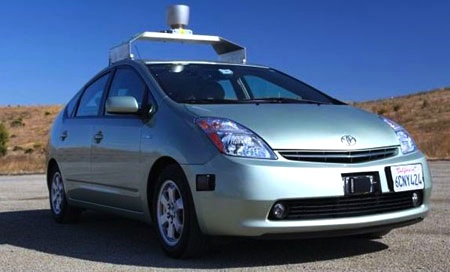
\includegraphics[width=0.42\textwidth, trim=4cm 00cm 1cm 0cm,clip]{graphics/google-laser-scan-cost.jpg}};
    \begin{scope}[x=(img.north east),y=(img.south west)] 
      \coordinate (velc) at (0.25, 0.10);
      \draw [very thick,red] (velc) ellipse (0.25 and 0.10);
      %\draw [->,red] (0,0) -- (1, 0) node {X};
      %\draw [->,red] (0,0) -- (0, 1) node {Y};
    \end{scope}
  \end{tikzpicture}
  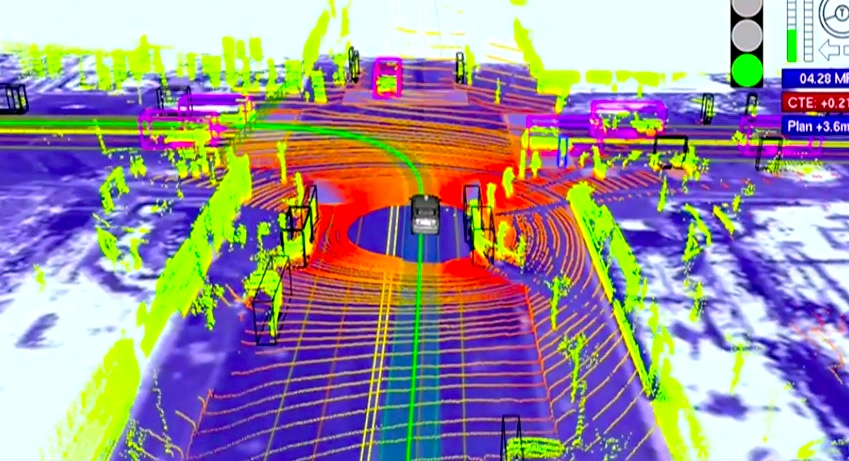
\includegraphics[width=0.50\textwidth, trim=3cm 00cm 3cm 0cm,clip]{graphics/google-laser-scan.jpg}
  \pause

  But Velodyne costs \tikz[remember picture] \node [anchor=north,inner sep=0] (cost) at (0,0) {\$75k};
\end{frame}

\begin{frame}{Can we do it with cameras? Stereo or Monocular}
  \begin{columns}
    \begin{column}{0.48\textwidth}
      \centering
      Left Camera\\
      \includemedia[label=stereoleft,
        width=\textwidth,
        activate=pageopen,
        addresource=graphics/upto61_quat.mp4,
        flashvars={
          source=graphics/upto61_quat.mp4
          &autoPlay=true
          &loop=true             % loop video
          &scaleMode=letterbox   % preserve aspect ratio while scaling the video
        }
      ]{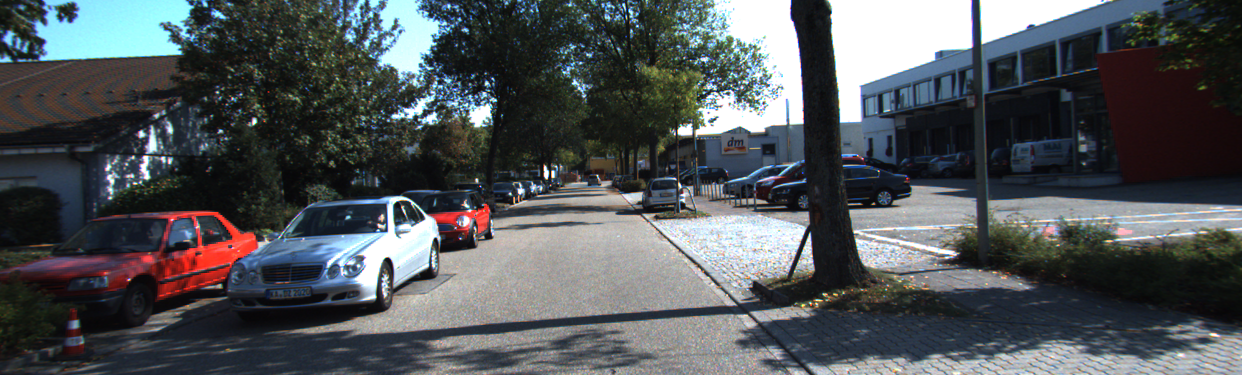
\includegraphics{graphics/0000000061_raw.png}}{VPlayer.swf}
    \end{column}
    \begin{column}{0.48\textwidth}
      \centering
      Right Camera\\
      \includemedia[label=stereoright,
        width=\textwidth,
        activate=pageopen,
        addresource=graphics/upto61_quat_right.mp4,
        flashvars={
          source=graphics/upto61_quat_right.mp4
          &autoPlay=true
          &loop=true             % loop video
          &scaleMode=letterbox   % preserve aspect ratio while scaling the video
        }
      ]{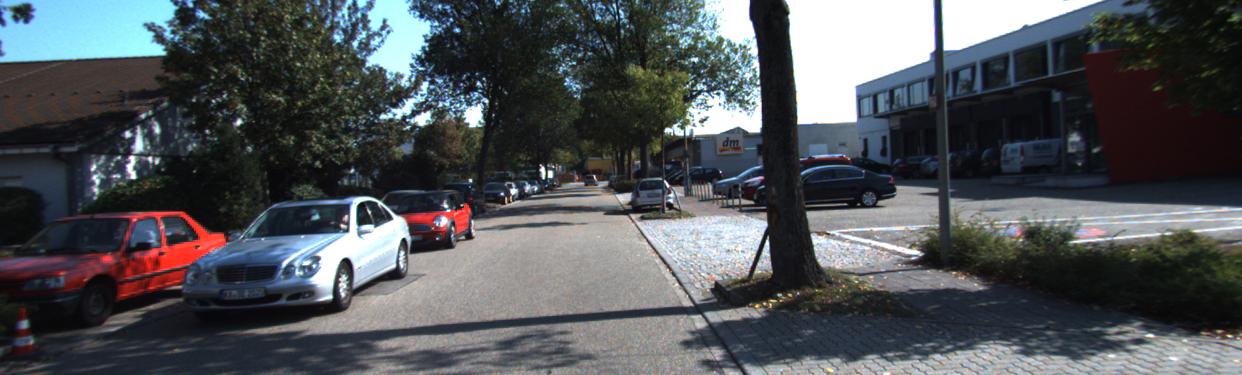
\includegraphics{graphics/0000000061_right.png}}{VPlayer.swf}
    \end{column}
  \end{columns}

  Stereo cameras need to be recaliberated

  And the depth range of stereo cameras are limited

  So after certain depth stereo is same as monocular
\end{frame}

% \begin{frame}{Problem}
%   % Notes: Spend around 30 sec on this slide
%   \centering
%   \begin{figure}
%     
\begin{tikzpicture}[	venn circle/.style={opacity=0.2,fill=#1,draw}]
  %\path[use as bounding box, draw] (-3*1.618, -3) rectangle (3*1.618, 3);

\path[venn circle=red] (0,0) ellipse (3*1.618 and 3);
\node at (0, 1.5) {Autonomous Driving};
\path[venn circle=blue] (0, -1) ellipse (2*1.618 and 2);
\node at (0, 0) {3D Localization};
\path[venn circle=green] (0, -2) ellipse (1.2* 1.618 and 1);
\node at (0, -2) {Occlusion modeling};
\end{tikzpicture}

%   \end{figure}
% \end{frame}
% This slide doesn't make it clear what problem we are trying to solve?  May be
% the slide that Manmohan made with an example image with cars and detections
% is better

% Should we have introduction slide that highlights our contributions?
% but we should have contributions to highlight them. Contributions are perhaps
% better with positive results but still. I don't think we should have negative
% results as a surprise. (It won't as they would have read the report.)

\begin{frame}{Sample input and output}
  \def\arrow{
    (0,0) -- ++(1,0)
    -- ++(0,1) -- ++(0.3, 0)
    -- ++(-0.8, 1) -- ++(-0.8, -1) -- ++(0.3, 0) -- ++(0, -1) }
    \begin{tikzpicture}
      \node[anchor=south west,inner sep=0] (image) at (0,0)
      {
        \includemedia[label=sampleinput,
          width=\textwidth,
          activate=pageopen,
          addresource=graphics/initonly_half.mp4,
          flashvars={
            source=graphics/initonly_half.mp4
            &autoPlay=true
            &loop=true             % loop video
            &scaleMode=letterbox   % preserve aspect ratio while scaling the video
          }
        ]{
        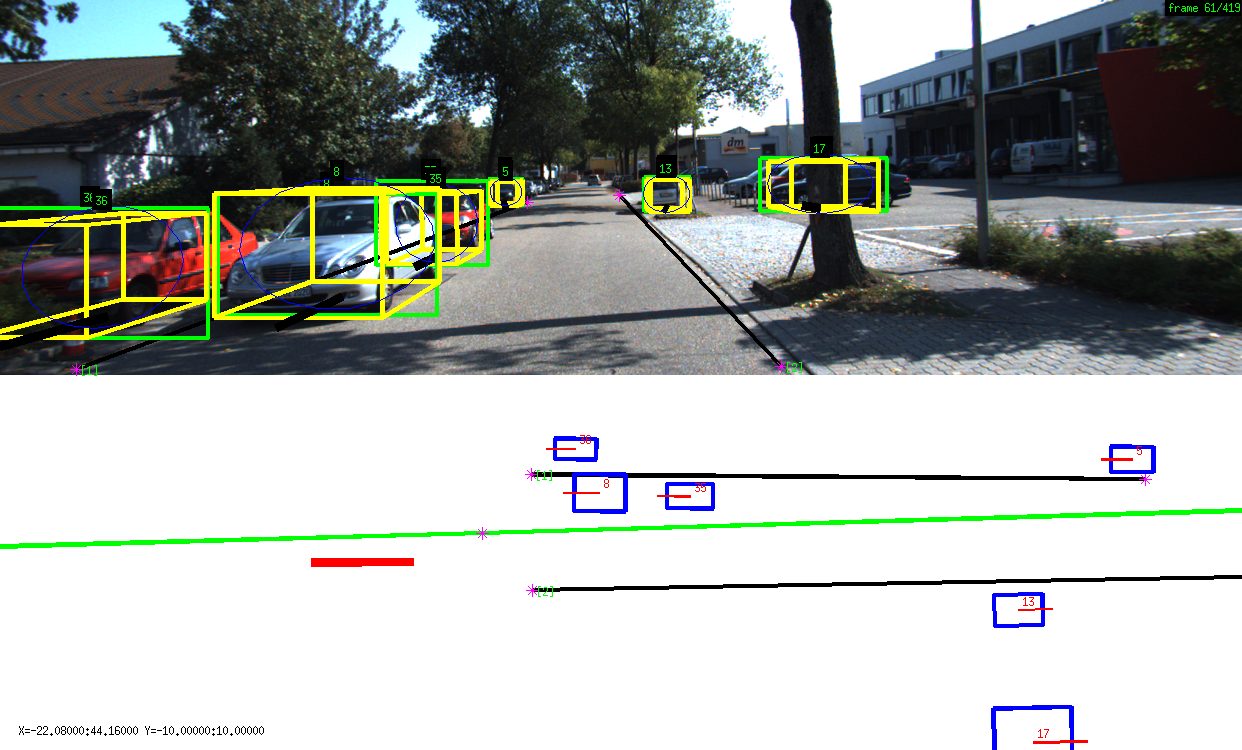
\includegraphics[width=\textwidth]{graphics/0000000061_bevdown.png}    }{VPlayer.swf}
      };
      \begin{scope}[x={(image.south east)},y={(image.north west)}]
        \fill[color=red,scale=0.05,shift={(10,11)},rotate=180,]\arrow;
      \end{scope}
    \end{tikzpicture}

\end{frame}

\begin{frame}{Intermediate inputs}
  % Need a flowchart that describes the input and desired output of the system
 \tikzset{/tikz/x=0.8cm,/tikz/y=0.8cm}
 \setlength{\units}{0.8cm}
  \scriptsize{
    \problemflowchart{}{}{}{}{}
  }
\end{frame}

\begin{frame}{Point tracks example}

  \includemedia[label=pointtracks,
    width=\textwidth,
    activate=pageopen,
    addresource=graphics/pointtracksvideo.mp4,
    flashvars={
      source=graphics/pointtracksvideo.mp4
      &loop=true             % loop video
      &autoPlay=true
      &scaleMode=letterbox   % preserve aspect ratio while scaling the video
    }
  ]{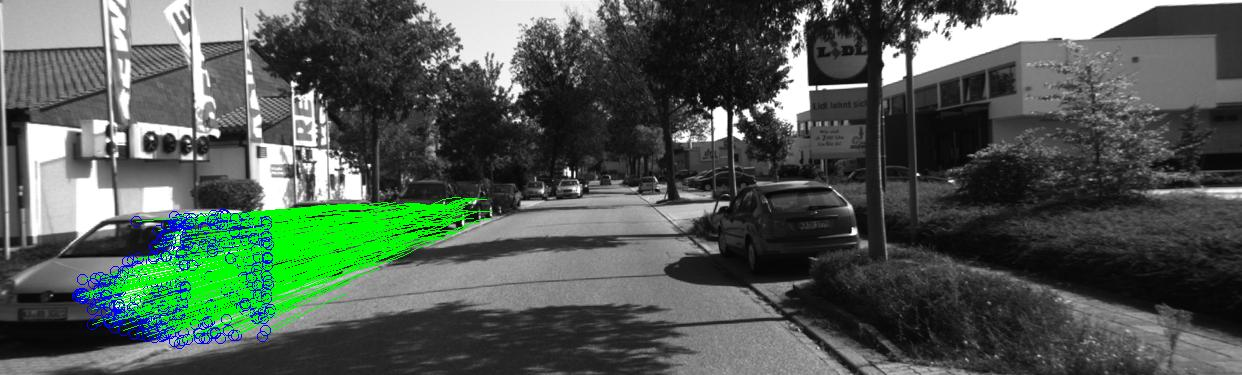
\includegraphics[width=\textwidth]{graphics/object_flow_tracks_4_000033.jpg}}{VPlayer.swf}
\end{frame}

% \begin{frame}{Problem}
%   \visible<-1>{
%     \begin{tikzpicture}
%       \node[anchor=south west,inner sep=0] (image) at (0,0)
%       {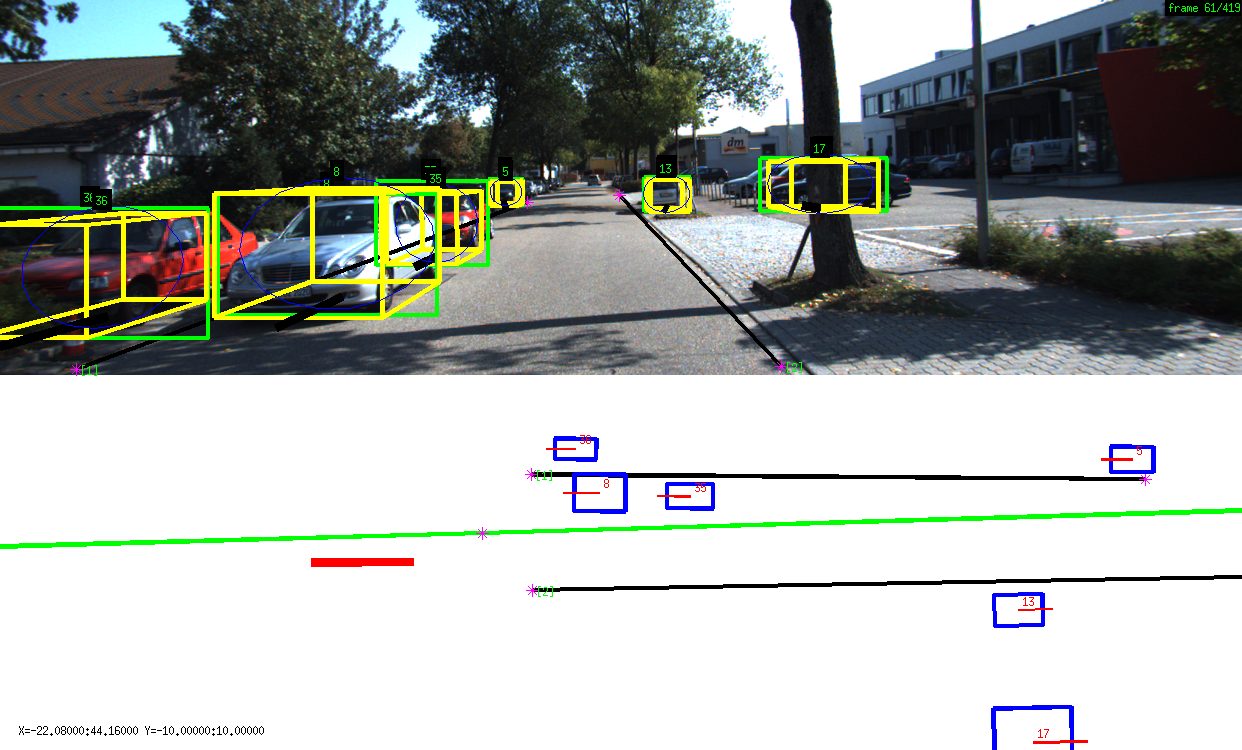
\includegraphics[width=\textwidth]{graphics/0000000061_bevdown.png}};
%       \fill[color=white] (image.south west) rectangle (image.east);
%     \end{tikzpicture}
%   }
% \end{frame}

\section{What has already been done?}

\paragraph{Occlusion handling in detection}
Several works in object detection consider occlusion by training a detector on visible parts of the object \cite{Gao_etal_2011}. Occlusion reasoning based on 2D image silhouettes is used to improve detection performance in \cite{Hsiao_Herbert_2012}. In contrast, our occlusion reasoning is based on 3D entities. In recent years, object detectors have also considered occlusion reasoning using 3D cues, often learned from a dataset of CAD models \cite{Pepik_etal_2012,Pepik_etal_2013,Xiang_Savarese_2013}. By necessity, such frameworks are often a discrete representation of occlusion behavior, for example, in the form of a collection of occlusion masks derived from object configurations discretized over viewpoint. In constrast to these works, our occlusion modeling is also fully 3D, but allows for a continuous representation. Further, to derive 3D information, we do not use CAD models, rather we derive a probabilistic formulation based on physical insights.

\paragraph{Occlusion handling in tracking}
Occlusions have also been handled in tracking-by-detection frameworks by considering occluder patterns in the image \cite{Kwak_etal_2012,Wu_Nevatia_2007}. A notable exception is the work of Milan et al.~\cite{Milan_etal_2014} that explicits models occlusion in the continuous domain to determine a visibility for each object in multi-target tracking. However, the occlusion model in \cite{Milan_etal_2014} is essentially the overlap of image projections of a Gaussian representation of the object. Our occlusion modeling is much more general in determining the probability of a point in space as belonging to an object. While it can also be used to determine a visibility ratio similar to \cite{Milan_etal_2014}, it can have far more general applications and can be quantitatively evaluated, as shown by our experiments on point track associations.

\paragraph{3D localization and scene understanding}
One of the central goals of 3D scene understanding is to localize the 3D positions and orientations of objects in complex scenes. For instance, using stereo imagery, several visual cues are combined in \cite{Geiger_etal_2014} to simultaneously determine object locations and a rough intersection topology. Similar to us, other works have also considered monocular frameworks. Notably, occlusions are explicitly handled in \cite{Wojek_etal_2013} by considering partial object detectors. A detailed part-based representation of objects based on annotated CAD models is used for monocular scene understanding in \cite{Zia_etal_2013,Zia_etal_2014}, which also allows reasoning about mutual occlusions between objects. In contrast to these works, our monocular framework uses a physical modeling of occlusion in continuous space, which makes it more general, extensible and amenable for continuous optimization.

\paragraph{Motion segmentation and multibody SFM}
An application for our occlusion modeling is to determine point track associations in scenes with multiple objects. For moving objects, this is within the purview of motion segmentation, which has been actively studied \cite{Tron_Vidal_2007,Rao_etal_2010}. This also motivates further applications such as object segmentation based on point trajectories \cite{Brox_Malik_2010}. Motion segmentation is also used within multibody structure from motion (SFM) frameworks \cite{Ozden_etal_2010,Kundu_etal_2011,Namdev2012}. In contrast to these works, our formulation does not distinguish between moving and static objects and also explicitly reasons about occlusions due to 3D object geometries for associating point tracks to individual objects.








% 
\section{Model}
\begin{frame}{Problem definition}
  \vspace{-0.5cm}
  \scriptsize{
    \problemflowchartnoraw{$\{\bb{i}\}_{i,t}$}{$\{\trackp{t}\}_{j,t}$}{$\{(\hat{\mathbf{n}}_t, h_t)\}_t$}{$\{c_t\}_{t}$}{$\{L_m(t)\}_{m,t}$}{\\$\{\state{i}{t}\}^*_{i,t} = \{\dimsn{i}, \relp{i}{t}\}_{i,t}$}{$\mathbb{E}$}{}
  }
\end{frame}
\begin{frame}{Graphical Model}
  \vspace*{-.5cm}
  \begin{center}
      \newcommand{\imagewidth}{0.9\textwidth}
      \usetikzlibrary{trees,shadows}
\providecommand{\imagewidth}{\textwidth}
\begin{tikzpicture}[
 line width=1.2,
variablenode/.style={circle,draw=red,fill=white,thick}]

% draw image
\node[anchor=south west,inner sep=0] (image) at (0,0)
{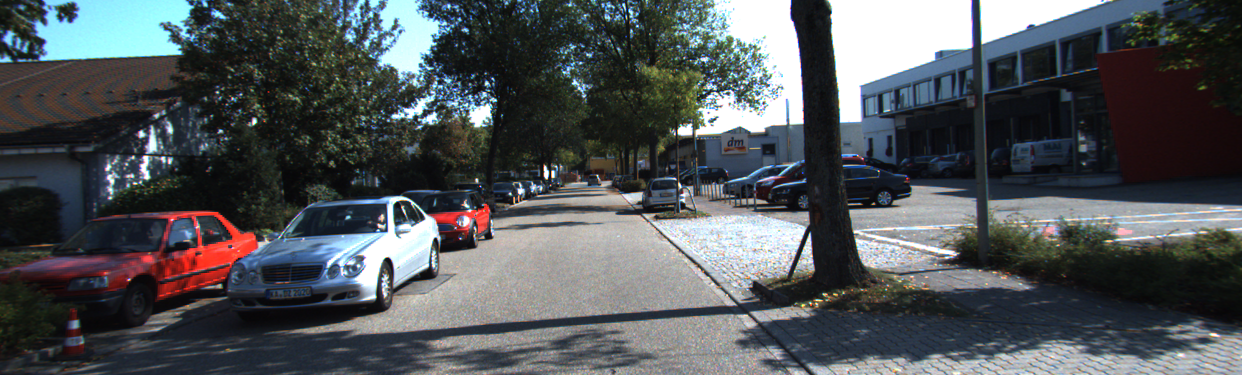
\includegraphics[width=\imagewidth]{graphics/0000000061_raw.png}};

    \begin{scope}[x={(image.south east)},y={(image.north west)}]
		\path (0.05, 0.3) node [variablenode] (x6) {\large{6}}
				    (0.25, 0.3) node [variablenode] (x2) {\large{2}}
				    (0.41, 0.45) node [variablenode,inner sep=3] (x1) {\tiny{1}}
				    (0.36, 0.39) node [variablenode,inner sep=3] (x5) {\small{5}}
				    (0.55, 0.4) node [variablenode,inner sep=3] (x3) {\small{3}}
					(0.63, 0.49) node [variablenode,inner sep=3] (x4) {\tiny{4}}
;
\draw (x6) -- (x2);
\draw (x5) -- (x2);
\draw (x1) -- (x5);
    \end{scope}
\end{tikzpicture}

  \end{center}
\end{frame}

\begin{frame}{Graphical Model}
  % Introduce the graphical model with a diagram and equations
  \begin{columns}
  \hskip-2cm
    \begin{column}[t]{0.9\textwidth}
      \tikzset{/tikz/x=0.9cm,/tikz/y=0.9cm}
      \usetikzlibrary{trees,shadows}
\providecommand{\Energy}[1]{E_{#1}}
\providecommand{\EnergyCol}{\Energy{col}}
\providecommand{\bb}[1]{d^{#1}(t)}
\providecommand{\trackp}[1]{u#1}
\providecommand{\pEnergy}[1]{E_{#1}}
\newcommand{\scenegraphicalmodel}{
  \begin{scope}[grow cyclic, line width=1.2,
      variablenode/.style={circle,circular drop shadow,draw=red,fill=white,thick},
      bboxfactor/.style= {rectangle,inner sep=2,fill=green!50!black,thick,text=green!50!black},
      collfactor/.style= {rectangle,inner sep=2,fill=blue,thick,text=blue},
      trackfactor/.style={rectangle,inner sep=2,fill=red,thick,text=red},
      obs/.style={fill=gray!30,draw=black,text=gray!30},
      prevf/.style={draw=green!20,text=gray},
      prevobsv/.style={draw=gray!10,fill=gray!1,text=gray},
      prevv/.style={draw=red!20,text=gray}
    ]
    \path[use as bounding box,clip] (-2.6, -5.5) rectangle (6.1,0.5);
    \draw (-2.5,-2.65) rectangle +(0.5,0.3);
    \draw (-2.0,-2.35) -- ++(0.15, 0.15) -- ++(0, -0.6) -- (-2.0, -2.65);
    \path
    (0, 0)  node [variablenode] (x6) {6}
    ++(0, -1.5) node [variablenode] (x2) {2}
    ++(2.5, 0)  node [variablenode] (x5) {5}
    +(.5, -2)   node [variablenode] (x3) {3}
    +(2.3, -3.5)   node [variablenode] (x4) {4}
    +(2.5, 0)  node [variablenode] (x1) {1}
    ;
    \visible<2-> {
      \path (x5)
      +(0, 1.5)  node [variablenode,obs] (u) {\tiny{1}}
      +(.2,0.9)  node {$\{\trackp{t}\}$};
    }

    % trackfactor
    \visible<2-> {
      \draw (x6) edge [bend left=40] node [trackfactor] (ft26) {\tiny{1}} (x2);
      \draw (ft26) edge [bend left=10] (u);
      \draw (x2) edge [bend left=35] node [trackfactor] (ft25) {\tiny{1}} (x5);
      \draw (ft25) edge (u);
      \draw (x5) edge [bend left=35] node [trackfactor] (ft51) {\tiny{1}} (x1);
      \draw (ft51) edge [bend right=35] (u);
    }

    % bboxfactors
    \visible<3->{
      \draw (x6) edge [bend right=40] node [bboxfactor] (f26) {\tiny{1}} (x2);
      \path (f26) +(-0.75,0) node [variablenode,obs] (d6) {\tiny{1}} 
      +(-.7,-.8)  node {$\bb{6}$};
      \draw (f26) edge (d6);
      \path (x2) ++(0,-1.25) node [variablenode,obs] (d2) {\tiny{1}} 
      +(-.8,0)  node {$\bb{2}$};
      \draw (x2) edge node [bboxfactor] {\tiny{1}} (d2);
      \draw (x2) edge [bend right=35] node [bboxfactor] (f25) {\tiny{1}} (x5);
      \path (x5) ++(-1.25,-1.25) node [variablenode,obs] (d5) {\tiny{1}} 
      +(.8,0)  node {$\bb{5}$};
      \draw (f25) edge (d5);
      \draw (x5) edge [bend right=35] node [bboxfactor] (f51) {\tiny{1}} (x1);
      \path (x1) ++(-1.25,-1.25) node [variablenode,obs] (d1) {\tiny{1}} 
      +(.8,0.2)  node {$\bb{1}$};
      \draw (f51) edge (d1);
      % \path (x3) ++(0,-1.25) node [variablenode,obs] (d3) {\tiny{1}} 
      % +(.8,0)  node {$\bb{3}$};
      % \draw (x3) edge node [bboxfactor] {\tiny{1}} (d3);
      % \path (x4) ++(0,1.25) node [variablenode,obs] (d4) {\tiny{1}} 
      % +(.8,0)  node {$\bb{4}$};
      % \draw (x4) edge node [bboxfactor] {\tiny{1}} (d4);
    }

    % colfactor
    \visible<4->{
      \draw (x6) edge node [collfactor] {\tiny{1}} (x2);
      \draw (x2) edge [] node [collfactor] {\tiny{1}} (x5);
      \draw (x5) edge [] node [collfactor] {\tiny{1}} (x1);
    }

    % Legend
    \visible<3->{
      \path (-1.75,-4.0) node (l1s) {} (-0, -4.0) node [anchor=west] (l1e) {$\EnergyBBox$};
      \draw (l1s) edge node [bboxfactor] {\tiny{1}} (l1e);
    }
    \visible<4->{
      \path (-1.75,-4.5) node (l2s) {} (0, -4.5) node [anchor=west] (l2e) {$\EnergyCol$};
      \draw (l2s) edge node [collfactor] {\tiny{1}} (l2e);
    }
    \visible<2->{
      \path (-1.75,-5.0) node (l3s) {} (0, -5.0) node [anchor=west] (l3e) {$\EnergyTrack$};
      \draw (l3s) edge node [trackfactor] {\tiny{1}} (l3e);
    }

  \end{scope}
}
\begin{tikzpicture}
  \scenegraphicalmodel
\end{tikzpicture}

    \end{column}
    \hspace{-2cm}
    \begin{column}[t]{0.4\textwidth}
      \vspace{-5cm}
      \scalebox{0.45}{
        \newcommand{\imagewidth}{2.125\textwidth}
        \usetikzlibrary{trees,shadows}
\providecommand{\imagewidth}{\textwidth}
\begin{tikzpicture}[
 line width=1.2,
variablenode/.style={circle,draw=red,fill=white,thick}]

% draw image
\node[anchor=south west,inner sep=0] (image) at (0,0)
{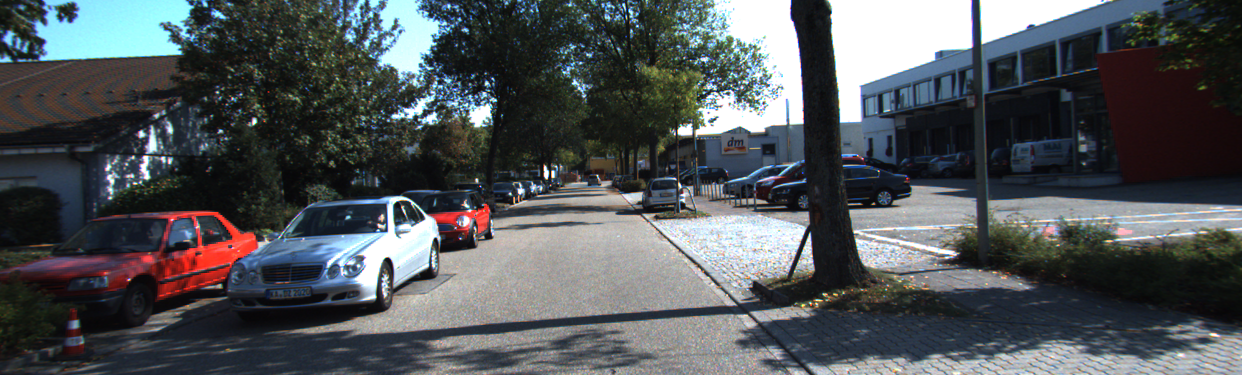
\includegraphics[width=\imagewidth]{graphics/0000000061_raw.png}};

    \begin{scope}[x={(image.south east)},y={(image.north west)}]
		\path (0.05, 0.3) node [variablenode] (x6) {\large{6}}
				    (0.25, 0.3) node [variablenode] (x2) {\large{2}}
				    (0.41, 0.45) node [variablenode,inner sep=3] (x1) {\tiny{1}}
				    (0.36, 0.39) node [variablenode,inner sep=3] (x5) {\small{5}}
				    (0.55, 0.4) node [variablenode,inner sep=3] (x3) {\small{3}}
					(0.63, 0.49) node [variablenode,inner sep=3] (x4) {\tiny{4}}
;
\draw (x6) -- (x2);
\draw (x5) -- (x2);
\draw (x1) -- (x5);
    \end{scope}
\end{tikzpicture}

      }
    \end{column}
  \end{columns}
\end{frame}

\begin{frame}{Graphical Model}
  % Introduce the graphical model with a diagram and equations
  \begin{columns}
  \hskip-2cm
    \begin{column}[c]{0.7\textwidth}
        \tikzset{/tikz/x=0.7cm,/tikz/y=0.7cm}
        \scriptsize{
          \usetikzlibrary{trees,shadows}
\providecommand{\Energy}[1]{E_{#1}}
\providecommand{\EnergyCol}{\Energy{col}}
\providecommand{\bb}[1]{d^{#1}(t)}
\providecommand{\trackp}[1]{u#1}
\providecommand{\pEnergy}[1]{E_{#1}}
\newcommand{\scenegraphicalmodel}{
  \begin{scope}[grow cyclic, line width=1.2,
      variablenode/.style={circle,circular drop shadow,draw=red,fill=white,thick},
      bboxfactor/.style= {rectangle,inner sep=2,fill=green!50!black,thick,text=green!50!black},
      collfactor/.style= {rectangle,inner sep=2,fill=blue,thick,text=blue},
      trackfactor/.style={rectangle,inner sep=2,fill=red,thick,text=red},
      obs/.style={fill=gray!30,draw=black,text=gray!30},
      prevf/.style={draw=green!20,text=gray},
      prevobsv/.style={draw=gray!10,fill=gray!1,text=gray},
      prevv/.style={draw=red!20,text=gray}
    ]
    \path[use as bounding box,clip] (-2.6, -4.5) rectangle (6.1,0.5);
    \draw (-2.5,-2.65) rectangle +(0.5,0.3);
    \draw (-2.0,-2.35) -- ++(0.15, 0.15) -- ++(0, -0.6) -- (-2.0, -2.65);
    \path
    (0, 0)  node [variablenode] (x6) {6}
    ++(0, -1.5) node [variablenode] (x2) {2}
    ++(2.5, 0)  node [variablenode] (x5) {5}
    +(.5, -2)   node [variablenode] (x3) {3}
    +(2.3, -2.5)   node [variablenode] (x4) {4}
    +(2.5, 0)  node [variablenode] (x1) {1}
    ;
    \path (x5)
    +(0, 1.5)  node [variablenode,obs] (u) {\tiny{1}}
    +(.2,0.9)  node {$\{\bu_j(t)\}$};

    % trackfactor
    \draw (x6) edge [bend left=40] node [trackfactor] (ft26) {\tiny{1}} (x2);
    \draw (ft26) edge [bend left=10] (u);
    \draw (x2) edge [bend left=35] node [trackfactor] (ft25) {\tiny{1}} (x5);
    \draw (ft25) edge (u);
    \draw (x5) edge [bend left=35] node [trackfactor] (ft51) {\tiny{1}} (x1);
    \draw (ft51) edge [bend right=35] (u);

    % bboxfactors
    \draw (x6) edge [bend right=40] node [bboxfactor] (f26) {\tiny{1}} (x2);
    \path (f26) +(-0.75,0) node [variablenode,obs] (d6) {\tiny{1}} 
    +(-.7,-.8)  node {$\textbf{d}^6(t)$};
    \draw (f26) edge (d6);
    \path (x2) ++(0,-1.25) node [variablenode,obs] (d2) {\tiny{1}} 
    +(-.8,0)  node {$\textbf{d}^2(t)$};
    \draw (x2) edge node [bboxfactor] {\tiny{1}} (d2);
    \draw (x2) edge [bend right=35] node [bboxfactor] (f25) {\tiny{1}} (x5);
    \path (x5) ++(-1.25,-1.25) node [variablenode,obs] (d5) {\tiny{1}} 
    +(.8,0)  node {$\textbf{d}^5(t)$};
    \draw (f25) edge (d5);
    \draw (x5) edge [bend right=35] node [bboxfactor] (f51) {\tiny{1}} (x1);
    \path (x1) ++(-1.25,-1.25) node [variablenode,obs] (d1) {\tiny{1}} 
    +(.8,0.2)  node {$\textbf{d}^1(t)$};
    \draw (f51) edge (d1);
    % \path (x3) ++(0,-1.25) node [variablenode,obs] (d3) {\tiny{1}} 
    % +(.8,0)  node {$\bb{3}$};
    % \draw (x3) edge node [bboxfactor] {\tiny{1}} (d3);
    % \path (x4) ++(0,1.25) node [variablenode,obs] (d4) {\tiny{1}} 
    % +(.8,0)  node {$\bb{4}$};
    % \draw (x4) edge node [bboxfactor] {\tiny{1}} (d4);

    % colfactor
    %% \draw (x6) edge node [collfactor] {\tiny{1}} (x2);
    %% \draw (x2) edge [] node [collfactor] {\tiny{1}} (x5);
    %% \draw (x5) edge [] node [collfactor] {\tiny{1}} (x1);

    % Legend
    \path (-1.75,-3.5) node (l1s) {} (-0, -3.5) node [anchor=west] (l1e) {$\Energy{detect}$};
    \draw (l1s) edge node [bboxfactor] {\tiny{1}} (l1e);
    % \path (-1.75,-4.5) node (l2s) {} (0, -4.5) node [anchor=west] (l2e) {$\EnergyCol$};
    %% \draw (l2s) edge node [collfactor] {\tiny{1}} (l2e);
    \path (-1.75,-4.2) node (l3s) {} (0, -4.2) node [anchor=west] (l3e) {$\EnergyTrack$};
    \draw (l3s) edge node [trackfactor] {\tiny{1}} (l3e);

  \end{scope}
}
\begin{tikzpicture}
  \scenegraphicalmodel
\end{tikzpicture}

        }
    \end{column}
    \hspace{-1.5cm}
    \vrule{}
    \begin{column}[c]{0.6\textwidth}
      \vspace{-1cm}
      \begin{center}
        \scalebox{0.45}{
          \newcommand{\imagewidth}{2.125\textwidth}
          \usetikzlibrary{trees,shadows}
\providecommand{\imagewidth}{\textwidth}
\begin{tikzpicture}[
 line width=1.2,
variablenode/.style={circle,draw=red,fill=white,thick}]

% draw image
\node[anchor=south west,inner sep=0] (image) at (0,0)
{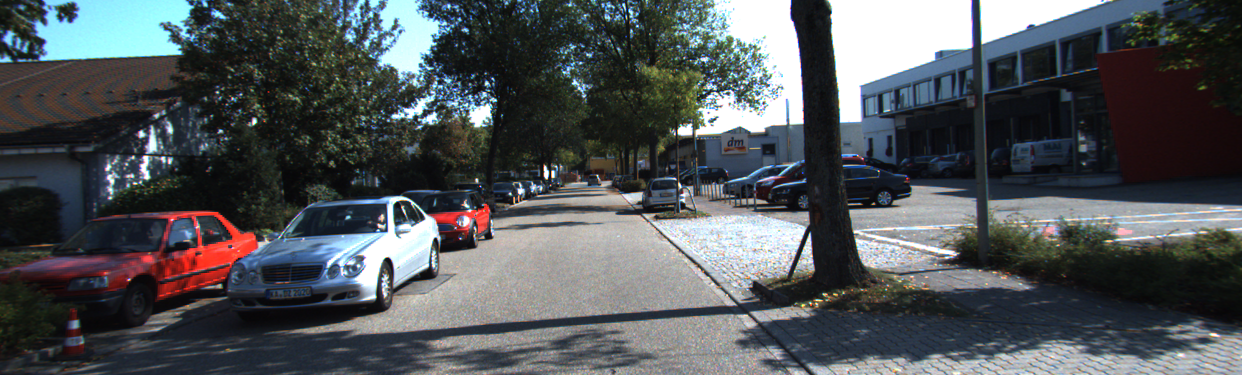
\includegraphics[width=\imagewidth]{graphics/0000000061_raw.png}};

    \begin{scope}[x={(image.south east)},y={(image.north west)}]
		\path (0.05, 0.3) node [variablenode] (x6) {\large{6}}
				    (0.25, 0.3) node [variablenode] (x2) {\large{2}}
				    (0.41, 0.45) node [variablenode,inner sep=3] (x1) {\tiny{1}}
				    (0.36, 0.39) node [variablenode,inner sep=3] (x5) {\small{5}}
				    (0.55, 0.4) node [variablenode,inner sep=3] (x3) {\small{3}}
					(0.63, 0.49) node [variablenode,inner sep=3] (x4) {\tiny{4}}
;
\draw (x6) -- (x2);
\draw (x5) -- (x2);
\draw (x1) -- (x5);
    \end{scope}
\end{tikzpicture}

        }
      \end{center}
      \tikzset{/tikz/x=0.8cm,/tikz/y=0.8cm}
      \usetikzlibrary{trees,shadows}
\providecommand{\Energy}[1]{E_{#1}}
\providecommand{\pEnergy}[1]{E_{#1}}
\providecommand{\EnergyCol}{\Energy{col}}
\providecommand{\relp}[2]{\mathbf{p}_{#1}({#2})}
\providecommand{\dimsn}[1]{\mathbf{B}^{#1}}
\providecommand{\bb}[1]{d^{#1}(t)}
\providecommand{\trackpit}[2]{\mathbf{u}^{(#1)}(#2)}
\begin{tikzpicture}[grow cyclic, line width=1.2,
    variablenode/.style={circle,circular drop shadow,draw=red,fill=white,thick,text=black},
    sizefactor/.style= {rectangle,inner sep=2,fill=magenta  ,thick,text=magenta},
    dynfactor/.style=  {rectangle,inner sep=2,fill=orange   ,thick,text=orange},
    lanefactor/.style= {rectangle,inner sep=2,fill=cyan    ,thick,text=cyan},
    trackfactor/.style={rectangle,inner sep=2,fill=red   ,thick,text=red},
    bboxfactor/.style= {rectangle,inner sep=2,fill=green!50!black,thick,text=green!50!black},
    level distance=30,
  obs/.style={fill=gray!30,text=gray!30,draw=black},
  prevf/.style={draw=green!20,text=gray},
  prevobsv/.style={draw=gray!10,fill=gray!1,text=gray},
  prevv/.style={draw=red!20,text=gray}
]
  \path[use as bounding box,clip] (-4.9, -4) rectangle (3.7,2.5);


  \path
  (-2.5,0) node[variablenode](dim) {2}
  +(-0.85, 0) node {$\dimsn{2}$};
  \visible<4->{
    \path (dim)
    +(-0.75,0.75) node[sizefactor](fsize){\tiny{2}}
    ;
    \draw (fsize) -- (dim);
  }

  \begin{scope}[line width=0.5]
    \path 
    % t-1 layer
    (1.5,1.5) node [variablenode] (xt1) {2}
    +(-0.20, 0.20) node[anchor=south east] {$\relp{2}{t-1}$}
  %  [counterclockwise from=-100,sibling angle=60]
  %  +(1.0, -1.0) node [factor,prevf] (flane1) {$E_{lane}$} 
  %  child { node [variablenode,obs,prevobsv] (l1) { $L_t$ } }
  %  child { node [ variablenode,obs,font=\footnotesize,prevobsv] (gps1) {GPS}}
  %  child { node [ variablenode,obs,font=\footnotesize,prevobsv] (map1) {Map}}

  %  [counterclockwise from=220]
  %  +(-1.0, -1.0) node[factor,prevf](fpt1) {$E_{pt}$}
  %  child { node[variablenode,obs,prevobsv](pt1){$u_t$} }

  %  [counterclockwise from=60,sibling angle=60]
  %  +(-1, 1.0) node[factor,prevf](fdet1){$E_{det}$} 
  %   child {
  %     node[variablenode,obs,prevobsv](gp1){$G_t$} 
  %   }
  %   child { node[variablenode,obs,prevobsv](Det1){$D_t$}
  %   }

    ;

  %\draw [gray](xt1) -- (fdet1) -- (dim);
  %\draw [gray](xt1) -- (flane1);
  %\draw [gray](xt1) -- (fpt1);
      
  \end{scope}

   %(0.5,1.0) node [dynfactor] (fdynx) {}
  %(1.95,1.8) node [factor,draw=gray,text=gray,minimum width=3] (fdynt) {$E_{d}$}

 %(0.2,2.0) node[factor](fhol) {$E_{hol}$}

  %(1, 0)  node[variablenode](theta){$\theta_t$}
  \draw
  (-1, 0)  node[variablenode](xt) {2}
  + (1.10, 0) node {$\relp{2}{t}$};
  \path 
  (-1.75, .75) node[bboxfactor](fdet){\tiny{2}} ;
  \path (-1.75, -.75) node[trackfactor] (fpt) {\tiny{2}};

  \draw (fpt) 
  ++(-90:1) node[variablenode,obs](pt){2} +(-.95,0) node {$\trackpit{2}{t}$} 
  ;
  \draw (xt) -- (fpt) -- (dim);
  \draw (fpt) -- (pt);
  \draw (fpt) edge [out=10,in=-110,gray] (xt1);
  \visible<3->{
    \draw (xt) edge node [dynfactor] (fdynx) {\tiny{2}} (xt1);
    \draw (xt) -- (fdynx) -- (xt1);
  }

  \visible<2->{
    \path (xt)
    ++ (0.75, -0.75) node [lanefactor] (flane) {\tiny{2}} ;
    %--
    %+ (-10:1) node [variablenode,obs] (l) {2} 
    % +(-10:1.8) node { $L_t$ } ;
    \draw (flane) --
    + (-45:1) node [ variablenode,obs,font=\footnotesize] (gps) {2} +(-60:1.7) node {$\{L_m\}$};
    %\draw (flane) -- +(-110:1)node [ variablenode,obs,font=\footnotesize] (map) {2} +(-110:1.7) node {Map};
    \draw (xt) -- (flane);
  }


 %++(65:1) node[variablenode,obs](gp){2} +(.75,0) node {$G_t$} ;
  \draw (fdet)
  --
  ++(90:1) node[variablenode,obs](Det){2} +(-.95,0) node {$\bb{2}$};
  \draw (xt) -- (fdet) -- (Det);
  
  %\path  (fpt) edge (theta);
  %\draw (fdet) -- (gp);
 %(0.2,2.0) node[factor](fhol) {$E_{hol}$}
  %\draw (xt) edge [bend left=40] node[factor] (fhol) {$E_{hol}$} (xt1);
  %\draw (fhol) -- (theta);  	  
  \draw (dim) -- (fdet);
  %\draw (theta) -- (flane);
  %\draw (theta) -- (fdynt) -- (theta1);
\coordinate (oneR) at (1.5,0);
\coordinate (oneRs) at (1,0);
  % Legend
  \visible<4->{
    \path (-3.8, -3.0) node (ls) {}
    ++(oneRs) node [anchor=west] (e1e) {$\EnergySize$};
    \draw (ls)  edge node [sizefactor] {\tiny{2}} (e1e) ;
  }
  \visible<3->{
    \path (e1e)
    ++(oneRs) node [] (e2s) {}
    ++(oneRs) node [anchor=west] (e2e) {$\EnergyDyn$};
    \draw (e2s) edge node [dynfactor] {\tiny{2}} (e2e) ;
  }
  \visible<2->{
    \path (e2e)
    ++(oneRs) node [] (e3s) {}
    ++(oneRs) node [anchor=west] (e3e) {$\EnergyLane$};
    \draw (e3s) edge node [lanefactor] {\tiny{2}} (e3e) ;
  }
\path (-3.8, -3.5)
  ++(oneRs) node [] (e4s) {}
  ++(oneRs) node [anchor=west] (e4e) {$\EnergyTrack$}
 ++(oneRs) node [] (e5s) {}
  ++(oneRs) node [anchor=west] (e5e) {$\EnergyBBox$}
  ;
  \draw (e4s) edge node [trackfactor] {\tiny{2}} (e4e) ;
  \draw (e5s) edge node [bboxfactor] {\tiny{2}} (e5e) ;
\end{tikzpicture}

      \end{column}
  \end{columns}
\end{frame}

\begin{frame}{Factorization}

\begin{align*}
  P(\{\state{i}{t}\} | \mathbb{E}) =
  \frac{1}{Z}P( \mathbb{E} | \{\state{i}{t}\})P(\{\state{i}{t}\})&.
\end{align*}
\begin{multline*}
  P(\{\state{i}{t}\} | \mathbb{E}) = \\
  \frac{1}{Z}
  \prod_{t=s}^{e}
  \left(
    \prod_{i,j: i \text{ occludes } j}
    {\colcol\underbrace{P(\state{i}{t}, \state{j}{t})}_{\text{col}}}
    {\colbbox\underbrace{P(\bb{i} | \state{i}{t}, \state{j}{t})}_{\text{bbox}}}
    {\coltrack\underbrace{P(\trackp{t} | \state{i}{t}, \state{j}{t})}_{\text{track}}}
\right)
\\
\left(
  \prod_{i=1}^{N}
  {\collane\underbrace{P(L_m(t) | \state{i}{t})}_{\text{lane}}}
  {\coldyn\underbrace{P(\state{i}{t} | \state{i}{t-1})}_{\text{dyn}}}
  {\colsize\underbrace{P(\state{i}{t})}_{\text{size}}}
\right)
  \enspace .
\end{multline*}
%

\end{frame}


\begin{frame}{Energy domain}

\begin{multline*}
  \hspace{-1cm}
  -\log{P(\{\state{i}{t}\} | \mathbb{E})} = 
  -Z' 
  + \sum_{t=s}^{e}
  \left(
    \sum_{i,j:i \text{ occludes } j}   
  \WEnergyCol 
   + \WEnergyBBox
   + \WEnergyTrack
\right)
  \\
  + \left(
  \sum_{i=1}^N 
  \WEnergyLane
  + \WEnergyDyn
  + \WEnergySize
\right)
  \enspace.
\end{multline*}
\begin{align*}
  \{\state{i}{t}\}^* &= \arg \min_{\{\state{i}{t}\}} - \log P(\{\state{i}{t}\} | \mathbb{E})\enspace.
\end{align*}
  
\end{frame}

\begin{frame}{Point Tracks energy (No Occlusion)}
  % Start with a simpler version of point track energy here
  \centering
  \begin{figure}
  

\usetikzlibrary{calc}

\begin{tikzpicture}[]
\begin{scope}[shift={(-2,0)},scale=1.5,]
\newcommand{\x}{1}
\drawframe{}
\renewcommand{\x}{2}
\drawframe{}
\coordinate (ut) at ($.2*(a2)+.2*(b2)+.6*(c2)$); 
\path[fill=red,draw]  (ut) circle (0.05);

\renewcommand{\x}{3}
\drawframe{}
\coordinate (ut1) at ($.6*(a3)+.2*(b3)+.2*(c3)$);
\path[fill=red,draw,] (ut1) circle (0.05);
\end{scope}

\caronroad{}
\coordinate (piinvut) at ($0.1*(a) + 0.3*(g) + 0.6*(d)$);
\path[fill=red,draw] (piinvut) circle (0.08);

\camera{}

\draw [->] (ut1) -- node (piinv) {} (piinvut) -- node (pi) {}  (ut);


% Equation
\path ($(a) + (-2,-1.5)$)  node (eq)  {$ 
    \EnergyTrackNoOcc = 
  \sum_{j \in \text{tracks}} \left\|\trackpj{t} - \projectionOf{\invProjectionOftm{\trackpj{t-1}}}\right\|^2$} ;
\coordinate (equt1) at ($0.2*(eq.north west)+0.8*(eq.north east) + (0, -0.2)$);
\draw(ut1) edge [->,thick,black!20!red,in=120,out=-90]  (equt1);

\coordinate (equt) at ($0.55*(eq.north west)+0.45*(eq.north east) + (0, -0.2)$);
\draw(ut) edge [->,thick,black!20!red,in=90,out=-90]  (equt);

\coordinate (eqpiinv) at ($0.4*(eq.north west)+0.6*(eq.north east) + (0, -0.2)$);
%\draw(piinvut) edge [->,thick,black!20!red,in=90,out=-90]  (eqpiinv);



\draw[dashed,thick,blue] (c3) -- (f);
\draw[dashed,thick,blue] (a3) -- (a);



\end{tikzpicture}

  \end{figure}
\end{frame}

% \begin{frame}{Point Tracks energy }
%   % Add the association fraction here, which requires occlusion modeling
% \end{frame}
% 
\begin{frame}{Occlusion modeling}
  Represent traffic participants as soft ellipsoids
  \centering
    \begin{tikzpicture}[x=0.95cm,y=0.95cm,3d/perspective eye={4,4,-10},ptstyle/.style={fill=#1,draw,circle,inner sep=1.5pt}]
    

% scale = xshift / (xshift + persepective eye z)
  \begin{scope}[shift={(1,1)},scale={10/11},facestyle/.style={fill=green!10,draw}]
    \acuboid

    \foreach \i/\j in {1/1,-2/2,-3/-3,-8/-2.7,-6/-3.1,-2.7/-6,-3.5/-9,3.5/-6,6/-3,6.2/3,4/0,0/5,-4/5,-6/3}{
      \pgfmathsetmacro{\color}{50*(6.2 - \i)/(6.2+8)}
      \path ($(a)+(0.1*\i,0.1*\j)$) node [ptstyle=red!\color!blue] (pta\i)   {};
      %\path +(0, \i) node {\coeffa} +(2, \i) node {\coeffb} +(4, \i) node {\coeffc} ;
    }
  \path [facestyle,shift={(-.5,-3)},rotate=60] (0,0) ellipse (1.2 and 0.7);
  \end{scope}
  \begin{scope}[facestyle/.style={fill=blue!10,draw}]
    \acuboid
    \foreach \i/\j in {-2/2,-3/-3,-8/-2.7,-6.1/-8.1,-8.7/-6,-3.5/-9,3.5/-6,6/-3,6.2/3,5/6,4/0,0/5,-4/5,-6/3}{
      \pgfmathsetmacro{\color}{50*(6.2 - \i)/(6.2+8.7) + 50}
      \path ($(a)+(0.1*\i,0.1*\j)$) node [ptstyle=red!\color!blue] (ptb\i)   {};
      %\path +(0, \i) node {\coeffa} +(2, \i) node {\coeffb} +(4, \i) node {\coeffc} ;
    }
  \path [facestyle,opacity=0.5,shift={(-.5,-3)},rotate=60] (0,0) ellipse (1.2 and 0.7);
  \end{scope}


    \begin{scope}[shift={(4,-2.5)}]
           \path [fill=blue!20,draw] (0,0) ellipse (1.2 and 0.7);
     \path [fill=green!20,draw] (3,0) ellipse (1.2 and 0.7);
     \coordinate (o) at (-2,-1);
     \draw(o) edge [->,very thick] node (xa) {} +(6, 0);
     \node at ($(xa) + (0, -0.2)$) {Depth from camera($\lambda$)};
     \draw(o) edge [->,very thick] node (ya) {} +(0, 2);
     \node [rotate=90]at ($(ya) + (-0.2, 0)$) {Probability};
    \draw [thick,blue]plot [smooth] coordinates {($(o)+(0,0.2)$) ($(o)+(0.2,0.2)$) ($(o) + (0.8, 1.8)$) ($(o)+(1.6,0.2)$) ($(o)+(3.2,0.2)$) 
      %($(o)+(3.8,1.8)$)  % Transmission prob corresponds to particular object
    ($(o)+(4.4,0.2)$) ($(o)+(6.4,0.2)$) };
    \draw [thick,red] plot [smooth] coordinates {($(o)+(0,1.8)$) ($(o)+(0.2,1.8)$) ($(o) + (0.8, 1.7)$) ($(o)+(1.4,0.2)$) ($(o)+(2.6,0.2)$) ($(o)+(3.2,1.8)$) ($(o)+(3.8,1.8)$) ($(o)+(4.4,0.2)$) ($(o)+(5.6,0.2)$) ($(o)+(6.1,1.8)$) };
   \draw [thick, blue] ($(o) + (0,-0.5)$) -- +(1,0) +(2,0) node {$P_{\text{reflection}}$};
   \draw [thick, red] ($(o) + (3,-0.5)$) -- +(1,0) +(2,0) node {$P_{\text{transmission}}$};

    \end{scope}
  \end{tikzpicture}

  % Transmission probability is product integral of over the depth
  % \[P^j_{\textit{transmission}}(\lambda) = \prod_{0}^{\lambda} (1 - \occft{\lambda \ray})^{d\lambda}\]
  Association probability for a point $j$ with object $i$: 
  \[\assocP = \Prefl\prod_{f}^{\lambda}\Ptransarg{\lambda \ray}^{d\lambda}\]
\end{frame}

\begin{frame}
  \centering
    \begin{tikzpicture}[x=0.95cm,y=0.95cm,3d/perspective eye={4,4,-10},ptstyle/.style={fill=#1,draw,circle,inner sep=1.5pt}]
    \begin{scope}[shift={(4,-2.5)}]
           \path [fill=blue!20,draw] (0,0) ellipse (1.2 and 0.7);
     \path [fill=green!20,draw] (3,0) ellipse (1.2 and 0.7);
     \coordinate (o) at (-2,-1);
     \draw(o) edge [->,very thick] node (xa) {} +(6, 0);
     \node at ($(xa) + (0, -0.2)$) {Depth from camera($\lambda$)};
     \draw(o) edge [->,very thick] node (ya) {} +(0, 2);
     \node [rotate=90]at ($(ya) + (-0.2, 0)$) {Probability};
    \draw [thick,blue]plot [smooth] coordinates {($(o)+(0,0.2)$) ($(o)+(0.2,0.2)$) ($(o) + (0.8, 1.8)$) ($(o)+(1.6,0.2)$) ($(o)+(3.2,0.2)$) 
      %($(o)+(3.8,1.8)$)  % Transmission prob corresponds to particular object
    ($(o)+(4.4,0.2)$) ($(o)+(6.4,0.2)$) };
    \draw [thick,red] plot [smooth] coordinates {($(o)+(0,1.8)$) ($(o)+(0.2,1.8)$) ($(o) + (0.8, 1.7)$) ($(o)+(1.4,0.2)$) ($(o)+(2.6,0.2)$) ($(o)+(3.2,1.8)$) ($(o)+(3.8,1.8)$) ($(o)+(4.4,0.2)$) ($(o)+(5.6,0.2)$) ($(o)+(6.1,1.8)$) };
   \draw [thick, blue] ($(o) + (0,-0.5)$) -- +(1,0) +(2,0) node {$P_{\text{reflection}}$};
   \draw [thick, red] ($(o) + (3,-0.5)$) -- +(1,0) +(2,0) node {$P_{\text{transmission}}$};

    \end{scope}
  \end{tikzpicture}

    \begin{align}
      f^i_{\text{occ}}(\bx) &= \frac{1}{1 + e^{-k(1 - d(\mathbf{x},\bp^{i}))}} \\
      P^{ij}_{\textit{reflection}} (\lambda) &= (\max \{0, \nabla {f^i_{\text{occ}}}(\lambda \ray)^\top \ray \})^2 \\
      P^j_{\textit{transmission}}(\lambda) &= \prod_i (1 - f^i_{\text{occ}}({\lambda \ray}))
    \end{align}
\end{frame}

\begin{frame}{Point tracks energy (With occlusion)}
  \centering
  \small{
  \begin{tikzpicture}[x=0.8cm,y=0.8cm,3d/perspective eye={4,4,-10},ptstyle/.style={fill=#1,draw,circle,inner sep=1.5pt}]
    

% scale = xshift / (xshift + persepective eye z)
  \begin{scope}[shift={(1,1)},scale={10/11},facestyle/.style={fill=green!10,draw}]
    \acuboid

    \foreach \i/\j in {1/1,-2/2,-3/-3,-8/-2.7,-6/-3.1,-2.7/-6,-3.5/-9,3.5/-6,6/-3,6.2/3,4/0,0/5,-4/5,-6/3}{
      \pgfmathsetmacro{\color}{50*(6.2 - \i)/(6.2+8)}
      \path ($(a)+(0.1*\i,0.1*\j)$) node [ptstyle=red!\color!blue] (pta\i)   {};
      %\path +(0, \i) node {\coeffa} +(2, \i) node {\coeffb} +(4, \i) node {\coeffc} ;
    }
  \path [facestyle,shift={(-.5,-3)},rotate=60] (0,0) ellipse (1.2 and 0.7);
  \end{scope}
  \begin{scope}[facestyle/.style={fill=blue!10,draw}]
    \acuboid
    \foreach \i/\j in {-2/2,-3/-3,-8/-2.7,-6.1/-8.1,-8.7/-6,-3.5/-9,3.5/-6,6/-3,6.2/3,5/6,4/0,0/5,-4/5,-6/3}{
      \pgfmathsetmacro{\color}{50*(6.2 - \i)/(6.2+8.7) + 50}
      \path ($(a)+(0.1*\i,0.1*\j)$) node [ptstyle=red!\color!blue] (ptb\i)   {};
      %\path +(0, \i) node {\coeffa} +(2, \i) node {\coeffb} +(4, \i) node {\coeffc} ;
    }
  \path [facestyle,opacity=0.5,shift={(-.5,-3)},rotate=60] (0,0) ellipse (1.2 and 0.7);
  \end{scope}


    \draw [->, very thick, draw=blue] (pta4) --  +(90:1) node [anchor=south,align=center] {$a^{1j}(\lambda) = 0$\\$a^{2j}(\lambda) = 1$};
    \draw [->, very thick, draw=red!50!blue] (pta-8) --  +(170:1.4) node [anchor=south,align=center] {$a^{1j}(\lambda) = 0.5$\\$a^{2j}(\lambda) = 0.5$};
    \draw [->, very thick, draw=red] ($(ptb-8)+(.5,-.8)$) --  +(-60:.8) node [anchor=north,align=center] {$a^{1j}(\lambda) = 1$\\$a^{2j}(\lambda) = 0$};
   \begin{scope}[shift={(4,-2)}]
     \path [fill=blue!20,draw] (0,0) ellipse (1.2 and 0.7);
     \path [fill=green!20,draw] (3,0) ellipse (1.2 and 0.7);
     \coordinate (o) at (-2,-1);
     \draw(o) edge [->,very thick] node (xa) {} +(6, 0);
     \node at ($(xa) + (0, -0.2)$) {Depth from camera ($\lambda$)};
     \draw(o) edge [->,very thick] node (ya) {} +(0, 2);
     \node [rotate=90]at ($(ya) + (-0.2, 0)$) {$a^{(1j)}(\lambda)$};
     \draw [thick,red] plot [smooth] coordinates {($(o)+(0,1.8)$) ($(o)+(0.2,1.8)$) ($(o) + (0.8, 1.7)$) ($(o)+(1.4,0.3)$) ($(o)+(3.8,0.2)$)($(o)+(4.4,0.1)$) ($(o)+(6.1,0.1)$)};
   \end{scope}
\end{tikzpicture}

  \begin{align*}
    \EnergyTrack = 
    \sum_{i \in \text{objects}}
    \sum_{j \in \text{points}}
    \int_{f}^{\infty}
      \assocP
      %\Ereproj(\lambda)
      \left\|\trackpj{t+1} - \projectionOft{\invProjectionOf{\trackpj{t}, \lambda}}\right\|^2
      d\lambda
  \end{align*}
}
\end{frame}

\begin{frame}{Association Experiment results}
\begin{table}
  \centering
  \begin{tabular}{lccc}
    \toprule
    Algorithm & All & Unoccluded cars & Occluded cars \\
    \midrule
    bounding box only                         & $0.18\pm0.01$          & $\color{red}0.04\pm0.003$  & $0.41\pm0.04$\\
    Using $\assocP{}$                         & $0.18\pm0.01$          & $0.05\pm0.003$           & $0.39\pm0.04$ \\
    Using $P^{(ij)}_{\text{assoc by reproj}}$ & $0.18\pm0.01$          & $0.06\pm0.003$           & $0.39\pm0.04$\\
    Using $P^{(ij)}_{\text{assoc}}$           & $\color{red}0.17\pm0.01$ & $0.05\pm0.003$           & $\color{red}0.38\pm0.04$\\
    \bottomrule
  \end{tabular}
  \caption{Error Metric: Average fraction of foreground points incorrectly associated to objects per sequence}
  %\caption{Association Experiment results. The error is in terms of fraction of points wrongly associated with objects, hence lower is better.}
\end{table}
  
\end{frame}

\begin{frame}{Association Experiment results}

\newlength{\tblimgwidth}
\setlength{\tblimgwidth}{0.090\textwidth}
\begin{figure}[!!t]
  \centering
  \begin{tabular}{cc@{}c@{\hspace{0.1cm}}c@{}c@{}}
    & Associations & Association Error & Associations & Association Error\\
    \rotatebox{90}{\hspace{1em} BBox}%
    & 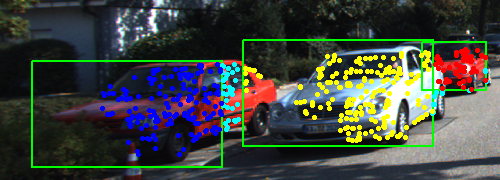
\includegraphics[height=\tblimgwidth]{results/0009_0000000060_point_assign_bbox2D_model-small.png}%
    & 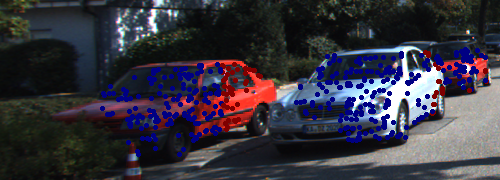
\includegraphics[height=\tblimgwidth]{results/0009_0000000060_point_assign_bbox2D_model_correct_incorrect-small.png}%
    & 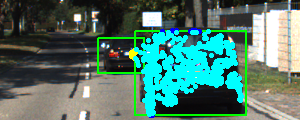
\includegraphics[height=\tblimgwidth]{results/0013_0000000060_point_assign_bbox2D_model-small.png}%
    & 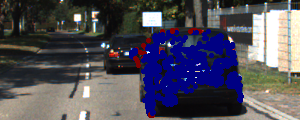
\includegraphics[height=\tblimgwidth]{results/0013_0000000060_point_assign_bbox2D_model_correct_incorrect-small.png}\\
    \rotatebox{90}{\hspace{1em} BM}%
    & 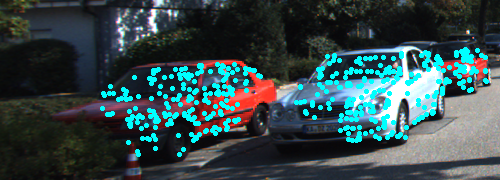
\includegraphics[height=\tblimgwidth]{results/0009_0000000060_point_assign_BroxAndMalik2010-small.png}%
    & 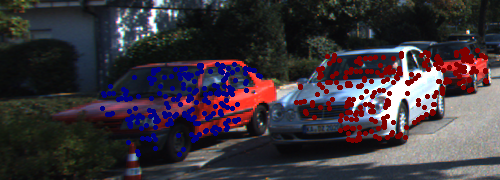
\includegraphics[height=\tblimgwidth]{results/0009_0000000060_point_assign_BroxAndMalik2010_correct_incorrect-small.png}%
    & 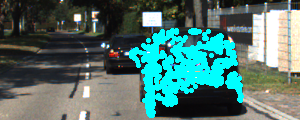
\includegraphics[height=\tblimgwidth]{results/0013_0000000060_point_assign_BroxAndMalik2010-small.png}%
    & 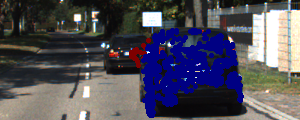
\includegraphics[height=\tblimgwidth]{results/0013_0000000060_point_assign_BroxAndMalik2010_correct_incorrect-small.png}\\
    \rotatebox{90}{\hspace{1em} RAS}%
    & 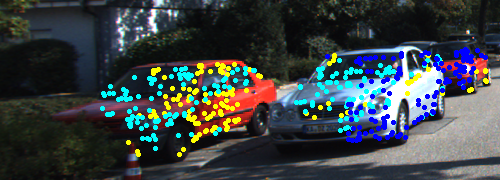
\includegraphics[height=\tblimgwidth]{results/0009_0000000060_point_assign_RAS-small.png}%
    & 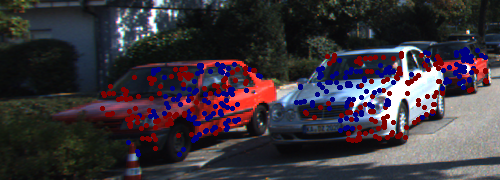
\includegraphics[height=\tblimgwidth]{results/0009_0000000060_point_assign_RAS_correct_incorrect-small.png}%
    & 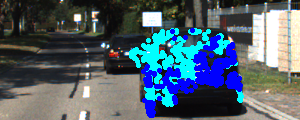
\includegraphics[height=\tblimgwidth]{results/0013_0000000060_point_assign_RAS-small.png}%
    & 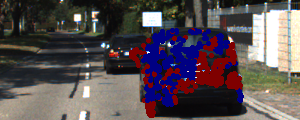
\includegraphics[height=\tblimgwidth]{results/0013_0000000060_point_assign_RAS_correct_incorrect-small.png}\\
    \rotatebox{90}{\hspace{1em} Ours}%
    & 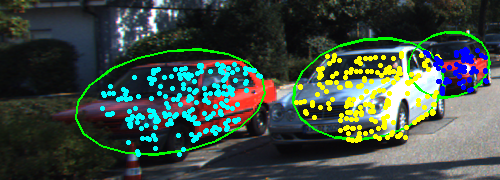
\includegraphics[height=\tblimgwidth]{results/0009_0000000060_point_assign_contPtTracks-small.png}%
    & 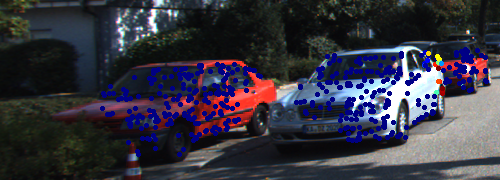
\includegraphics[height=\tblimgwidth]{results/0009_0000000060_point_assign_contPtTracks_correct_incorrect-small.png}%
    & 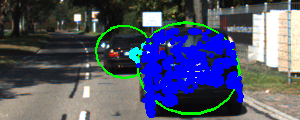
\includegraphics[height=\tblimgwidth]{results/0013_0000000060_point_assign_contPtTracks-small.png}%
    & 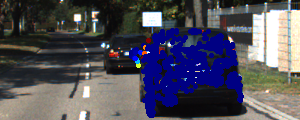
\includegraphics[height=\tblimgwidth]{results/0013_0000000060_point_assign_contPtTracks_correct_incorrect-small.png}
  \end{tabular}
  \vspace{-0.3cm}
\label{fig:qualitative}
\vspace{-0.3cm}
\end{figure}
  
\end{frame}

\begin{frame}
\begin{table}
\begin{tabular}{lrrrr}
  \toprule
  & Ours & BBox & BM & RAS\\
  \midrule
  Dyn. and occ. tracks        & \textbf{13.2} & 21.3 & 30.9 & 30.1 \\
  Occluded tracks             & \textbf{15.7} & 19.8 & 39.5 & 37.8 \\
  Dynamic tracks              & \textbf{06.6} & 11.4 & 15.3 & 17.7 \\
  All tracks                  & \textbf{08.6} & 12.6 & 21.9 & 21.5 \\
  \bottomrule
\end{tabular}
\caption{\small Mean association errors on different sets of input point tracks over all sequences of KITTI dataset. Errors are in terms of average fractions of foreground points incorrectly associated to objects per sequence.}
\label{tab:meanAssoc}
\end{table}
\end{frame}

% Consider packing other energies in fewer slides 
\begin{frame}{Bounding box energy (No Occlusion)}
  % 
  \centering
  \begin{figure}
    \providecommand{\Energy}[1]{E_{#1}}
\providecommand{\pEnergy}[1]{E_{#1}}
\providecommand{\EnergyCol}{\Energy{col}}
\providecommand{\relp}[2]{\mathbf{p}_{#1}({#2})}
\providecommand{\dimsn}[1]{\mathbf{B}^{#1}}
\providecommand{\projectionOf}[1]{\pi_{\relp{i}{t}}\left(#1\right)}
\providecommand{\projectionOft}[1]{\pi_{\relp{i}{t+1}}\left(#1\right)}
\providecommand{\bbt}[2]{\mathbf{d}^{#1}(#2)}

\usetikzlibrary{calc}

\begin{tikzpicture}[]

\newcommand{\x}{1};
\drawframe;
\node (ld\x) at ($(a\x) +(0,-1)$) {$\bbt{i}{t=T}$};
\draw[->,black!40!green,very thick] ($.5*(d\x)+.5*(a\x)$) -- (ld\x);

\renewcommand{\x}{2};
\drawframe;
\node (ld2) at ($(a2) +(0,-1)$) {\dots};

\renewcommand{\x}{3};
\drawframe;
\node (ld\x) at ($(a\x) +(0,-1)$) {$\bbt{i}{t=1}$};
\draw[->,black!40!green,very thick] ($.5*(d\x)+.5*(a\x)$) -- (ld\x);


\caronroad{}


\camera{}

% Equation
\path ($(a) + (0,-2)$)  node (eq)  {$\EnergyBBoxNoOcc = \left\|\projectionOf{\dimsn{i}}-\bbt{i}{t}\right\|^2$} 
			+(-0.4, 0.1) node (eqp) {}
            + (0.4, 0.2) node (eqb) {}
            +(1.3,0.2) node (eqd) {};

% Label detections
\path (ld3) edge[->,thick,black!40!green,in=90,out=0] (eqd);

% Label 3D bbox
\path ($.5*(a)+.5*(b)$) edge[->,thick,blue,in=90,out=-90] (eqb);

\draw[dashed,thick,blue] (c3) -- (f);
\draw[dashed,thick,blue] (a3) -- (a);


\path ($0.5*(c0)+0.5*(c2)$) edge[->,thick,black,in=90,out=-90] (eqp);

\end{tikzpicture}

  \end{figure}
\end{frame}

\begin{frame}{Bounding box energy with occlusion}
  \centering
  \usetikzlibrary{intersections}
\begin{tikzpicture}[3d/perspective eye={4,4,-10}]
  \begin{scope}[shift={(0.7,0.9)},scale={10/11},facestyle/.style={fill=green!10,draw=green,thick}]
    \acuboid

  \end{scope}

  \draw [draw=green!50!black,very thick] (b) rectangle (h);
  \path  [name path=gbbox] (b) |- (h);
  \draw [name path=cross1,draw=green!50!black,very thick] (b) -- (h) ;
  \draw [name path=cross2,draw=green!50!black,very thick] (d-| b) -- (b -| h) ;
   \coordinate (gh) at (h);
   \coordinate (gb) at (b);
   \coordinate (gdpb) at (d-|b);

  \begin{scope}[opacity=0.6,facestyle/.style={fill=blue!20,draw=blue!20,very thick}]
    \acuboid
  \end{scope}

  \draw [name path=bbbox,draw=blue!50!black,very thick] (b) rectangle (h) ;

   \path [name intersections={of=cross1 and bbbox,by=E}];
   \path [name intersections={of=gbbox and bbbox,by=F}];
   \path [name intersections={of=cross1 and cross2,by=C}];
   \node [anchor=north east] at (gh) {A};
   \node [anchor=north west] at (gdpb) {D};
   \node [anchor=south west] at (gb) {C};
   \node [anchor=south east] at (gb -| gh) {B};
   \node [anchor=south] at (C) {E};
   \fill [red!30] (gh) -- (E) -- (b) -- (F) -- cycle;
   \node [anchor=west] at ($(C) + (1,0)$) {$v_{AD} = \frac{\text{area(\tikz \node [rectangle,inner sep=0,fill=red!30,text=red!30] {0};)}}{\text{area}(\bigtriangleup AED)}$};
\end{tikzpicture}

  \begin{align}
    \mathcal{V} &= \text{diag}([v_{AB}, v_{BC}, v_{CD}, v_{DA}])\\
    \EnergyBBox &= \left\| \mathcal{V} \left(\projectionOf{\dimsn{i}}-\bbt{i}{t}\right) \right\|^2
  \end{align}
\end{frame}

\begin{frame}{Lane information}
  \begin{columns}[c]
    \begin{column}{0.5\textwidth}
      \begin{itemize}
        \item Use OpenStreetMaps to extract lane geometry
          \begin{itemize}
            \item Use GPS coordinates aligned with SFM egomotion
            \item Automatically filter out small lanes and side streets
          \end{itemize}
        \item Annotated lanes (to be replaced by lane detector)
      \end{itemize}
    \end{column}
    \begin{column}{0.5\textwidth}
      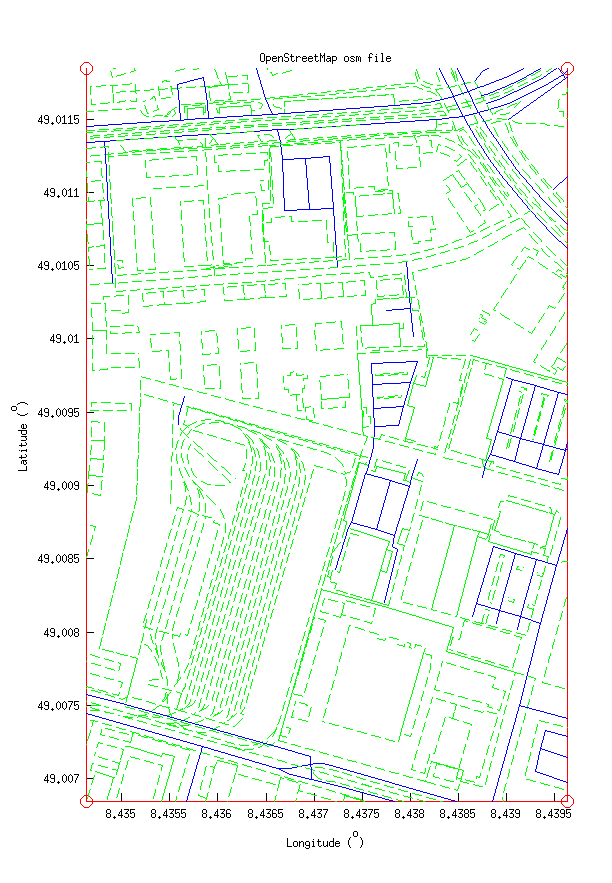
\includegraphics[width=\columnwidth]{graphics/mapimg.png}
    \end{column}
  \end{columns}

\end{frame}

\newcommand{\carbev}{
  \coordinate (ra) at (1,0.2);
  \coordinate (rb) at (2,0.7);
  \draw [thick,blue] (ra) rectangle (rb);
  \draw [thick,black] let \p1 = (ra), \p2 = (rb) in ($.5*(\x1, \y2) + .5*(\x1, \y1) + (-0.2,0)$) -- ($.5*(ra)+.5*(rb)$);
}
\begin{frame}{Lane energy}
      \centering
  \begin{columns}
    \begin{column}[t]{0.5\textwidth}
      \centering
      Low Energy

      \begin{tikzpicture}
        \path [use as bounding box] (-.5,-0.5) rectangle (2.5,1.5);
        \draw [thick,green] (0,0) -- (2,0);
        \carbev
      \end{tikzpicture}
    \end{column}
    \begin{column}[t]{0.5\textwidth}
      \centering
      High Energy

      \begin{tikzpicture}
        \path [use as bounding box] (-.5,-0.5) rectangle (2.5,1.5);
        \draw [thick,green] (0,0) -- (2,0);
        \begin{scope}[rotate around={60:(1.5,0.55)}]
          \carbev
        \end{scope}
      \end{tikzpicture}
    \end{column}
  \end{columns}
  \begin{align}
    \label{eq:laneOrientationEnergy}
    \EnergyLane &= 
    \sum_{m \in M_{\text{close}}}
    (1 - \ori{i}{t} \cdot \text{TAN}(L_{m}(k), \pos{i}{t}) )
    \LaneUncertainty{\pos{i}{t}}
    \\
    \LaneUncertainty{\pos{i}{t}} &=
    \frac{1}{1 + exp(-q(w_{\text{road}} - \text{DIST}(L_{m}(k), \pos{i}{t})))}
  \end{align}
    
\end{frame}

\begin{frame}{Collision energy}
  \begin{columns}
    \begin{column}[t]{0.5\textwidth}
      \centering
      Low Energy

      \begin{tikzpicture}
        \path [use as bounding box] (-.5,-0.5) rectangle (2.5,1.5);
        \draw [thick,green] (0,0) -- (2,0);
        \carbev
        \begin{scope}[shift={(0.9,-0.7)}]
          \carbev
        \end{scope}
      \end{tikzpicture}
    \end{column}
    \begin{column}[t]{0.5\textwidth}
      \centering
      High Energy

      \begin{tikzpicture}
        \path [use as bounding box] (-.5,-0.5) rectangle (2.5,1.5);
        \draw [thick,green] (0,0) -- (2,0);
        \carbev
        \begin{scope}[rotate around={-30:(1.5,0.55)},shift={(0.9,0)}]
          \carbev
        \end{scope}
      \end{tikzpicture}
    \end{column}
  \end{columns}
  \begin{align}
    \EnergyCol &= -\log\left(
  A_{ij}
  e^{-\frac{1}{8}
    \left(\pos{i}{t} - \pos{j}{t}\right)^\top
    P^{-1}
    \left(\pos{i}{t} - \pos{j}{t}\right)
    }
    \right)
  \end{align}
  where 
  \begin{align}
    A_{ij} &= \frac{|\Sigma_i|^\frac{1}{4}|\Sigma_j|^\frac{1}{4}}
    {|P|^\frac{1}{2}}\\
    P &= \frac{1}{2}\Sigma_i + \frac{1}{2}\Sigma_j
  \end{align}
\end{frame}

\begin{frame}{Transition energies}
  \begin{columns}
    \begin{column}{0.5\textwidth}
      \centering
      Low Energy\\
      \begin{tikzpicture}
        \draw [thick,green] (0.5,0) -- (3.5,0);
        \begin{scope}[shift={(0,0.1)},rotate around={-10:(1.5,0.55)}]
          \carbev
        \end{scope}
        \begin{scope}[shift={(1.2,0)},every path/.style={dotted}]
          \carbev
        \end{scope}
      \end{tikzpicture}
    \end{column}
    \begin{column}{0.5\textwidth}
      \centering
      High Energy\\
      \begin{tikzpicture}
        \draw [thick,green] (0.5,0) -- (3,0);
        \carbev
        \begin{scope}[shift={(0.3,-0.4)},every path/.style={dotted}]
          \carbev
        \end{scope}
      \end{tikzpicture}
      
    \end{column}
  \end{columns}
\begin{align}
  \label{eq:totalPosTransitionEnergy}
  \EnergyDynHol &= 1 - \left(\ori{i}{t-1} \cdot \frac{\pos{i}{t} - \pos{i}{t-1}}{\|\pos{i}{t} - \pos{i}{t-1}\|})\right)^2 \\
  \EnergyDynOri &= \|\ori{i}{t} - \ori{i}{t-1}\|^2\\ 
  \EnergyDynVel &= \|(\pos{i}{t} - 2\pos{i}{t-1}) + \pos{i}{t-2}\|^2
\end{align}
\end{frame}


\begin{frame}{Size prior}
  
\newcommand{\badsizeconfig}{
\begin{tikzpicture}[3d/perspective eye={8,4,-10}]
\begin{scope}[facestyle/.style={draw=green!50!black,very thick}]
  \acuboid
  \node at ($(f)+(.0,.3)$) {\color{green!50!black}$\expDimsn$};
\end{scope}
\begin{scope}[shift={(0,0.3,1)},facestyle/.style={draw=red,very thick}]
  \long\def\zlen{2.2}
  \long\def\ylen{.5}
  %\acuboid
  \providecommand{\xmin}{-2}
  \providecommand{\xlen}{1}
  \providecommand{\ymin}{-2}
  \providecommand{\ylen}{1}
  \providecommand{\zmin}{-2}
  \providecommand{\zlen}{1}
  \pgfmathsetmacro{\ymax}{\ymin+\ylen}
  \pgfmathsetmacro{\xmax}{\xmin+\xlen}
  \pgfmathsetmacro{\zmax}{\zmin+\zlen}
  \coordinate (a) at (3d cs:\xmax,\ymax,\zmin);
  \coordinate (b) at (3d cs:\xmax,\ymax,\zmax);
  \coordinate (c) at (3d cs:\xmax,\ymin,\zmax);
  \coordinate (d) at (3d cs:\xmax,\ymin,\zmin);
  \coordinate (h) at (3d cs:\xmin,\ymin,\zmin);
  \coordinate (e) at (3d cs:\xmin,\ymax,\zmin);
  \coordinate (f) at (3d cs:\xmin,\ymax,\zmax);

  \draw [facestyle] (a) -- (b) -- (c) -- (d) -- cycle;
  \draw [facestyle] (a) -- (b) -- (f) -- (e) -- cycle;
  \draw [facestyle] (a) -- (d) -- (h) -- (e) -- cycle;

  \node at ($(h)+(-.2,-.2)$) {\color{red}$\dimsn{i}$};
\end{scope}
\end{tikzpicture}
}
\newcommand{\goodsizeconfig}{
\begin{tikzpicture}[3d/perspective eye={4,4,-10}]
\begin{scope}[facestyle/.style={draw=green!50!black,very thick}]
  \acuboid
  \node at ($(b)+(.2,.2)$) {\color{green!50!black}$\expDimsn$};
\end{scope}
\begin{scope}[scale=1.08,facestyle/.style={draw=red,very thick}]
  \acuboid
  \node at ($(h)+(-.2,-.2)$) {\color{red}$\dimsn{i}$};
\end{scope}
\end{tikzpicture}
}

% \begin{document}
% \badsizeconfig
% \goodsizeconfig
%   
% \end{document}

  \begin{columns}
    \begin{column}{0.5\textwidth}
      \centering
      Low Energy\\
      \goodsizeconfig
    \end{column}

    \begin{column}{0.5\textwidth}
      \centering
      High Energy\\
      \badsizeconfig
    \end{column}
  \end{columns}
\begin{align}
  \label{eq:totalSizeEnergy}
  \EnergySize &= (\dimsn{i} - \expDimsn)^\top\Sigma_{\expDimsn}^{-1}(\dimsn{i} -
  \expDimsn)
\end{align}
\end{frame}

% 
\section{Inference}
We use two methods for inference, Metropolic Hastings and block coordinate descent. We briefly describe the inference algorithms for completeness.

\section{Metropolis Hastings}
Metropolis Hastings requires a \emph{transition probability} $Q(\map'|
\map^r)$, that depends on current sample $\map^r$ and guides
the random walk in the high-dimensional space. We randomly sample a point
$\map'$ from from $Q(.)$ and it is either accepted or rejected based on the
\emph{acceptance probability} $a$:
\begin{align}
  a = \frac{P(\map')Q(\map^r| \map')}
  {P(\map^r)Q(\map'| \map^r)}
  \enspace,
\end{align}
where $P(\map)$ is joint probability of the model at point $\map$.

If $a \ge 1$, then the new point $\map'$ is accepted otherwise it is accepted
with probability $a$. Here acceptance means that the point in the next
iteration is taken as the sampled point otherwise the earlier point is retained.

\section{Block Coordinate Descent}

We use block coordinate descent algorithm on our factor graph, by iteratively
minimizing the energy with respect to only a subset (block) of random 
variables. We choose to divide the blocks along the
variable types like dimension, yaw and position. Hence we iteratively minimize the energies with respect to dimension variables, then with respect to yaw variables and then with respect to position variables. Since we know the dependence of parts of our energy on specific variables, thanks to factor graph formulation, we can minimize the energies corresponding to the given set of variables.

% 
\section{Results}
\begin{frame}{Qualitative results: Our system}
  % Show some impressive qualitative results that are better than naive
  % initialization
  \centering
  \includemedia[label=allenergies,
    width=\linewidth,height=0.6\linewidth, % 16:9
    activate=pageopen,
    addresource=graphics/allenergies_2.mp4,
    flashvars={
      source=graphics/allenergies_2.mp4
      &loop=true             % loop video
      &scaleMode=letterbox   % preserve aspect ratio while scaling the video
    }
  ]{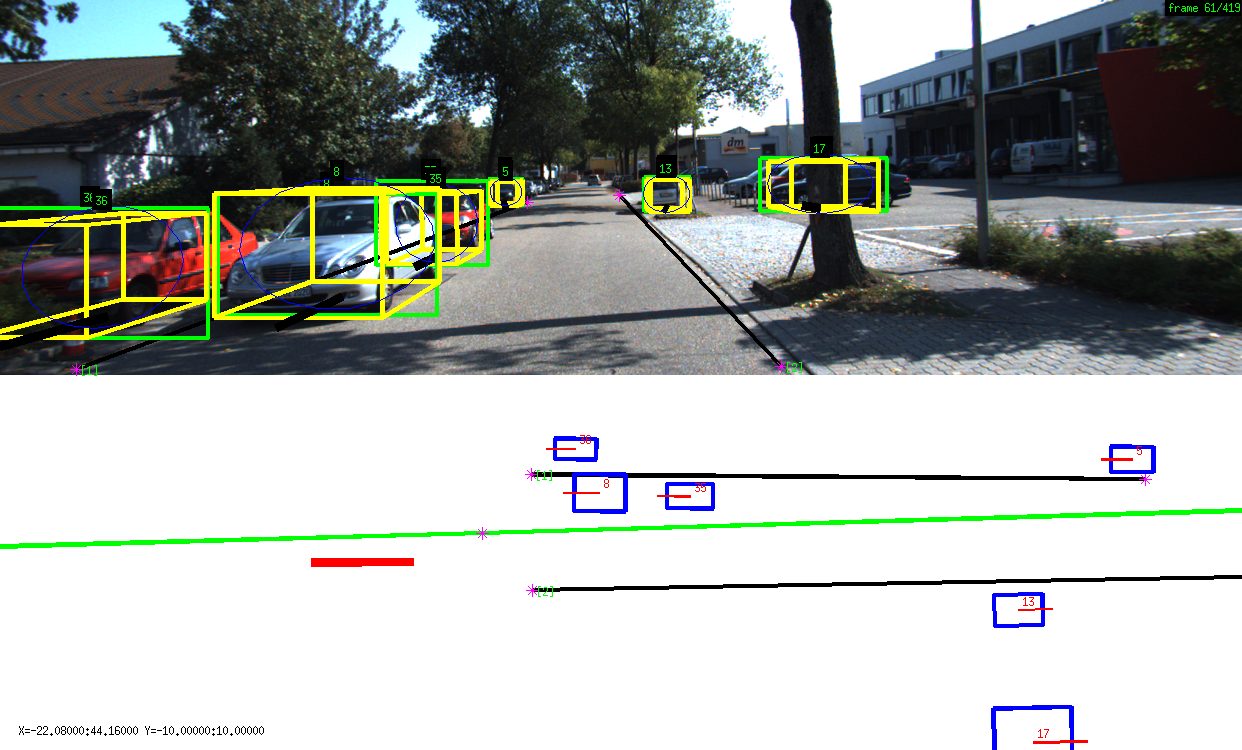
\includegraphics{graphics/0000000061_bevdown.png}}{VPlayer.swf}
\end{frame}

\begin{frame}{Quantitative results}

  \begin{tabular}{lrr}
    \toprule
    Method & t & dim \\
    \midrule
    Point cloud fit
    & 6.87 & 4.02\\
    Initialization
    & 5.61 & 3.23\\
    $\EnergyTrackNoOcc + \EnergyBBoxNoOcc +\EnergySize+\EnergyDyn$ 
    & 3.95  & 1.72\\        
    $\EnergyTrackNoOcc + \EnergyBBox +\EnergySize+\EnergyDyn$        
    & 4.81  & 2.16\\        
    $\EnergyTrack + \EnergyBBoxNoOcc +\EnergySize+\EnergyDyn$      
    & 4.05  & {\bf 1.59}\\        
    $\EnergyTrack + \EnergyBBox +\EnergySize+\EnergyDyn$             
    & {\bf 3.24}  & 2.16\\
    \bottomrule
  \end{tabular}
  
\end{frame}

\begin{frame}{Future work}
  \begin{itemize}
    \item Speedup inference
    \item Simplify graph by \cite{chow1968approximating} tree approximation
    \item Use belief propagation for faster inference on trees
  \end{itemize}
  
\end{frame}

\begin{frame}{Conclusion}
    Our occlusion aware 3D modeling improves association\\
    ... but requires more work to show improvement on localization
\end{frame}

% 
\section{Thank you}
\begin{frame}{Bibliography}
\bibliography{presentation}
\bibliographystyle{plainnat}
\end{frame}

\end{document}
